\chapter{Study of dark count rate and correlated noise in a DarkSide SiPM}
\label{ch:anal}

In the previous chapters we studied the impact of electrical noise in the
procedure to identify and measure the signal produced by an incident photon.
However the photodetector itself produces pulses which are not directly caused
by an external photon. Such pulses can be produced independently of incident
light, as in the case of thermally-generated avalanches, or result from
secondary-avalanche generation mechanisms triggered by a primary avalanche. In
the latter case we refer to them as correlated noise.

We will give a brief explanation and classification of the SiPM noise and then
characterize it on a specific Tile from the LFoundry production, using laser
data collected with the LNGS test stand. In doing this, we rely on several of
the tools introduced in the previous chapters.

There are two goals in characterizing the SiPM noise. First, a quantitative
model of the noise is needed for the DarkSide20k simulation, and we will
provide an estimate of the parameters that can be used to simulate the behavior
of the most recent version of the DarkSide TPC photosensors. Second, using the
fast frontend electronics of the TPC PDMs we can classify noise pulses by
looking at their amplitude and time distribution. This provides a validation
sample against which one can test more indirect noise characterization methods,
necessary, e.g., when relying on slower front-end electronics. This is a topic
of interest for monitoring applications, e.g., for the sensors installed in the
VETO, which feature the same Tile as the TPC ones, but slower electronics.

\section{Theory}
\label{sec:analtheory}

In \autoref{ch:darkside} and~\ref{ch:snr} we briefly introduced the silicon
photomultiplier (SiPM). We now recap and expand the explanation, mainly
following \cite[ch.~3]{savarese2018}. For a general introduction to
semiconductor detectors, but not the SiPM, see \cite[ch.~11]{knoll2010}.

The difference between a SiPM and older kinds of semiconductor detectors is
that the SiPM has a binary response: the amplitude of the output is not
proportional to the energy released by the detected particle. In this sense
they are analogous to Photomultiplier Tubes (PMTs), because they are designed
to detect just the presence of a photon with high efficiency ($\sim\SI{50}\%$).

A SiPM is composed by a grid of \emph{microcells}. The microcells are Single
Photon Avalanche Photodiodes (SPADs). A SPAD is a photodiode operated in
reverse bias above its breakdown voltage in series with a \emph{quenching
resistor}. Since the bias is above breakdown, if a current starts in the
photodiode it will be self sustaining and would normally destroy the diode. The
resistor in series lowers the potential difference on the diode when a current
flows through it, stopping the current because the diode goes below breakdown,
so the output pulse will have duration and amplitude uniquely determined by the
resistor and the capacitance of the diode junction, independently of the
initial release of energy that triggered the current.

The difference between the bias and the breakdown voltage is called
\emph{overvoltage}, and is often indicated with the unit ``\si{VoV}'' meaning
``Volt overvoltage''.

The output from all the microcells is summed analogically, so if multiple microcells are
triggered simultaneously, the amplitude of the output pulse is discretized and
proportional to the number of fired microcells. As we already said in
\autoref{ch:snr}, we will use the term ``PE'', standing for ``photoelectrons'',
as a unit when indicating the number of microcells corresponding to a pulse.

\subsection{SiPM noise}
\label{sec:sipmnoise}

The initial creation of an electron-hole pair that starts the avalanche in the
photodiode can either be caused by an absorbed photon or by a thermal
fluctuation. The latter case happens randomly with probability that depends on
temperature, and the resulting rate of random pulses is called \emph{dark count
rate}, where ``dark'' stands for the fact that these pulses occur even when the
photodiode is kept isolated from light.

A ``primary'' pulse, either thermally- or photon-generated, can induce other
pulses, that can themselves recursively produce additional pulses in the same
way. The main mechanisms for the proliferation of pulses are listed here and
illustrated in \autoref{fig:sipmnoise}:

\begin{description}

    \item[Afterpulse (AP)] During the avalanche, charge carriers can remain
    trapped into impurities and imperfections of the crystal. They are released
    afterwards at random times, starting another avalanche in the same microcell.
    
    \item[Direct cross talk (DiCT)] A photon emitted by an avalanche can
    trigger a nearby microcell.
    
    \item[Delayed cross talk (DeCT)] Instead of hitting directly another microcell,
    the photon can be absorbed in the shared crystal substrate and generate
    a hole that travels up until it passes through a microcell and triggers an
    avalanche there.
    
    \item[Delayed afterpulse] In the latter case, if the hole hits the
    originating microcell, we call it delayed afterpulse instead of DeCT.

\end{description}

\begin{figure}
    
    \centering
    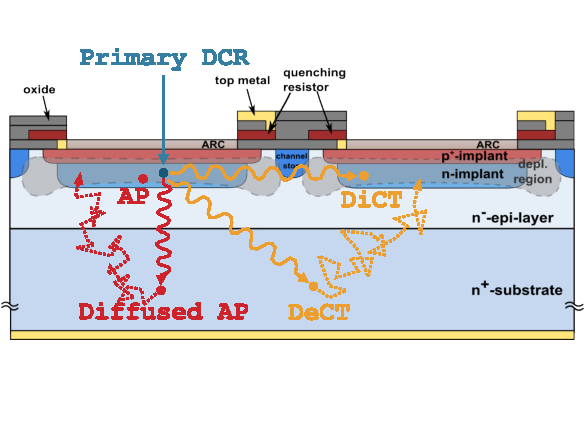
\includegraphics[width=0.85\textwidth]{sipmnoise}
    
    \caption{\label{fig:sipmnoise} Schematic of SiPM noises overlaid on the
    cross section of the device: AP (afterpulse), DiCT (direct cross talk),
    DeCT (delayed cross talk). From \cite[53]{savarese2018}.}
    
\end{figure}

To remove ambiguity, the DCR as we intend here may be called ``primary DCR'',
as in \cite[fig.~3]{acerbi2017} for example, to be distinguished from the total
rate with includes the correlated noise produced by the primary DCR.

The microcells have a pitch of \SI{35}{\micro m}, so the DiCT pulse starts
within \SI1{ps} of the originating pulse, while as we saw in \autoref{ch:snr}
even just the peak of the pulse lasts $\sim\SI{10}{ns}$. This means that the
effect of the DiCT is multiplying the height of the pulse by an integer factor,
because the overlapping pulses are well aligned. Afterpulses and DeCT, instead,
can arrive with a significative delay, and thus can be distinguished from the
originating pulse.

The reason why we classify separately the delayed pulses, instead of having an
overarching category of ``delayed noise'', is that afterpulses have a different
amplitude. The shape of the pulse is a sharp peak followed by an exponentially
decaying tail. This tail is due to the capacitance of the reverse-biased
junction that recharges through the quenching resistor after being discharged
inside the diode by the avalanche. A pulse generated in the same microcell
before its complete recharge can only use up the charge present in that moment.
Delayed cross talk, instead, has full amplitude because it involves a different
microcell. See \autoref{fig:sipmnoiseampl}.

A category of correlated noise we did not mention, and will not study, is
external cross talk (eCT). It is like DiCT, but mediated by an external object.
For example, when a SiPM is attached to a scintillator, the correlated noise
increases due to photons emitted by the avalanches that are reflected back by
the scintillator \cite[8]{gola2014}. We make the assumption that our data is
free from eCT. An anecdotal estimate of the expected eCT probability in
DarkSide20k at \SI{9}{VoV} is \SI{10}\%.

\begin{figure}
    
    \centering
    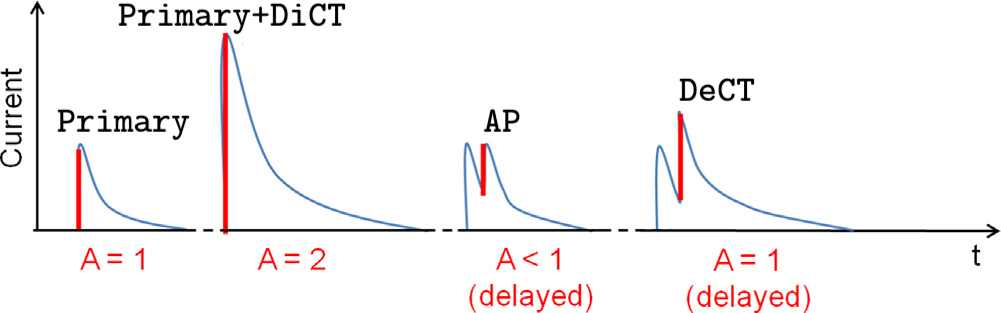
\includegraphics[width=0.85\textwidth]{sipmnoiseampl}
    
    \caption{\label{fig:sipmnoiseampl} Schematic of noise pulses. From
    \cite[4]{nagy2014}.}
    
\end{figure}

\stracka{Qui assumi che uno possa leggersi la Tesi di Savarese. In realta' non
e' pubblica. \upshape Risposta: è open access, ho controllato, non cito mai
cose che non sono pubbliche}

From \cite[tab.~3.1~p.~62]{savarese2018} we report typical values for the DCR
and correlated noise probabilities in FBK devices similar to the LFoundry
device we characterize here. The dark count rate, converted from rate per area
to rate per PDM (area \SI{25}{cm^2}), is \SI{25}{cps}. The correlated noise
probabilities are: DiCT \SI{17}\%, AP \SI{17}\%, DeCT \SI{1.5}\%. These are the
probabilities for a \SI1{PE} pulse to generate at least one pulse of the
specified category.

Among correlated noise mechanisms, in the following we focus on DiCT and AP.
For the DeCT we will just give a very rough estimate, since we are not able to
select cleanly this class of pulses. From \cite[fig.~3.8~p.~54]{savarese2018},
in fact, we can see that DeCT occurs within \SI{50}{ns} and our analysis is not
sensitive to secondary pulses with delays below \SI{100}{ns}. Also, since the
probability is smaller than the other noise modes, we completely neglect second
order effects due to DeCT.

\subsection{DiCT model}
\label{sec:dicttheory}

Like primary pulses, noise pulses can themselves produce other noise pulses. We
can imagine quite complicated interactions, for example: a DiCT induces a DeCT
on the original cell, thus producing a ``secondary'' delayed afterpulse. Or a
DiCT induces an afterpulse that induces a DiCT on the originating cell, again
with an afterpulse as final outcome. If the probabilities involved are small
enough, we should get by with the following simplifying assumption: that for
each pulse, the DiCT involves new cells that were not previously involved in
the chain, and the distribution of the number of DiCT at each step is fixed.

For the generation model of DiCT, we follow \cite{vinogradov2012}. Even when
multiple DiCT steps are chained, the combined delay is very small compared to
the duration of the pulse, so the overall effect of the complete DiCT ``tree''
is still to multiply the amplitude of the first pulse. This means that at the
end we just need to know the distribution of the total number of consecutive
DiCT.

For the single DiCT step, we consider two distributions: Bernoulli and Poisson.
In the first case we assume that a cell can induce a DiCT in at most just
another cell. In the second, we assume that there is a infinite population of
other cells, each with a fixed probability to be triggered. Clearly these two
cases are ``opposite'' approximations. In the first case, the distribution of
the total number of PE $k$ is Geometric. If $p$ is the probability of
generating a DiCT at each step, the distribution is
%
\begin{equation}
    P_G(k;p) = p^{k-1}(1-p), \quad k \ge 1, \quad p \in [0,1).
    \label{eq:geometric}
\end{equation}
%
Note that the conventional parametrization of the Geometric distribution is
different, with $p$ and $1 - p$ interchanged. We use this formulation because
it is more intuitively comparable with the other case. If the branching
distribution is Poisson with mean $\mu_B$, the total distribution is the Borel,
%
\begin{equation}
    P_B(k;\mu_B) = e^{-k\mu_B} \frac {(k\mu_B)^{k-1}} {k!},
    \quad k \ge 1, \quad \mu_B \in [0,1).
    \label{eq:borel}
\end{equation}
%
If it were $\mu_B \ge 1$, $k$ would diverge with nonzero probability.

The formula for the mean is formally the same for the two distributions,
%
\begin{equation}
    E[k] = \frac 1 {1 - p} = \frac 1 {1 - \mu_B},
\end{equation}
%
thus, since the interesting quantity is the amount of excess pulses due to
noise, it makes sense to compare the two distributions when $p = \mu_B$. We
make such comparison in \autoref{fig:geomborel} for $p = \mu_B = 0.5$. We note
that the Borel distribution has higher probability in the no-DiCT case, and at
the same time a fatter tail, while being lower in the few-DiCT cases.

\begin{figure}
    
    \widecenter{\includempl{figgeomborel}}

    \figcaption{geomborel}{Top panels: comparison of the geometric and Borel
    distributions (Equations~\ref{eq:geometric} and~\ref{eq:borel}), used for
    the total number of pulses in the DiCT tree, including the initial pulse.
    Bottom panels: geometric and generalized Poisson
    (Equations~\ref{eq:geompoisson} and~\ref{eq:genpoisson}), for the total
    number of PE when the number of initial pulses is Poisson distributed. The
    right panels are the same plots on the left in logarithmic scale.}
    
\end{figure}

Since we use laser data, there can be multiple photons hitting the SiPM. The
light is diffused before reaching the photodetector (see \autoref{ch:data}), so
we expect at most one photon per cell, and thus a Poisson distribution for the
initial number of fired cells. So for the analysis we will need the
distribution of the total number of PE $n \ge 0$ for an initial
Poisson-distributed number of cells, each with its DiCT tree.

For the geometric model, the resulting distribution is called geometric Poisson
or Pólya-Aeppli. Let $\mu_P$ be the initial Poisson mean. The probability mass
function $P_{GP}$ can be computed with this recursion \cite[5]{nuel2008}:
%
\begin{align}
    P_n &\equiv P_{GP}(n;\mu_P,p), \\
    z &\equiv \mu_P \frac{1-p}p, \\
    P_0 &= e^{-\mu_P}, \\
    P_1 &= e^{-\mu_P} zp, \\
    P_n &= \frac{2n - 2 + z}n p P_{n-1} + \frac{2-n}n p^2 P_{n-2}.
    \label{eq:geompoisson}
\end{align}

For the Borel model, the distribution is the generalized Poisson:
%
\begin{equation}
    P_{BP}(n;\mu_P,\mu_B)
    = e^{-(\mu_P + n\mu_B)} \frac {\mu_P(\mu_P + n\mu_B)^{n-1}} {n!}.
    \label{eq:genpoisson}
\end{equation}

The means of the two distributions are, unsurprisingly, $\mu_P/(1-p)$ and
$\mu_P/(1-\mu_B)$. Note that for $n = 0$ the probabilities are equal, since
of course the cross talk does not affect the case with zero initial pulses.

The referenced article finds a much better agreement with the Borel model when
looking at the tails of the PE distribution for DiCT only
\cite[p.~3~fig.~1]{vinogradov2012}, while it does not find a visible difference
for the Poisson+DiCT distribution with $\text{PE} \le 11$
\cite[p.~4~fig.~2]{vinogradov2012}.

\subsection{Afterpulse model}
\label{sec:aptheory}

For the afterpulses we have to model not just the number of pulses, but also
their temporal distribution and amplitude.

In a generally accepted explanation, afterpulses are produced by carriers
trapped during the avalanche that get released afterwards \cite{nagy2014},
\cite{cova1991}. The release of trapped carriers is a thermodynamical process
regulated by the potential difference that the carriers must overcome to jump
out of their traps. This means that it also depends on the external bias. If
there were only one kind of trap, the carrier release temporal distribution
would be exponential. However we expect to have various possible trapping
energy levels, so the distribution is in general a mixture of exponentials.

The released carriers also have a non-unitary probability of generating an
avalanche. This probability also depends on the electric field and thus on the
bias, like the release probability. The bias in turn depends on the recharge
state of the cell, thus deforming the exponential distribution for low delays.
While \cite[2]{nagy2014} tries to keep into account this deviation by
multiplying the afterpulse temporal distribution with the fraction of recovered
charge
%
\begin{equation}
    1 - \exp\left(-\frac{\Delta t}{\tau_\text{rec}}\right),
    \label{eq:recfactor}
\end{equation}
%
where $\tau_\text{rec}$ is the exponential scale of the pulse shape tail, and
$\Delta t$ is the delay from the primary pulse, other authors
\cite[4]{garutti2014} parametrize the time distribution with pure exponentials.
However, we notice from \cite[p.~5~fig.~11]{nagy2014}, reported here in
\autoref{fig:nagyap}, that they do not actually have data at low delays to test
the accuracy of their model, since the relatively high threshold they use for
peak finding truncates the afterpulse distribution at $\approx\SI{80}{ns}$.
Even though the recharge time is $\tau_\text{rec} = \SI{207}{ns}$, thus making
the correction term \eqref{eq:recfactor} significative even above the temporal
cut, by looking at the plotted histogram we think that a vanilla exponential
with a different amplitude and scale could fit as well.

\begin{figure}
    
    \centering
    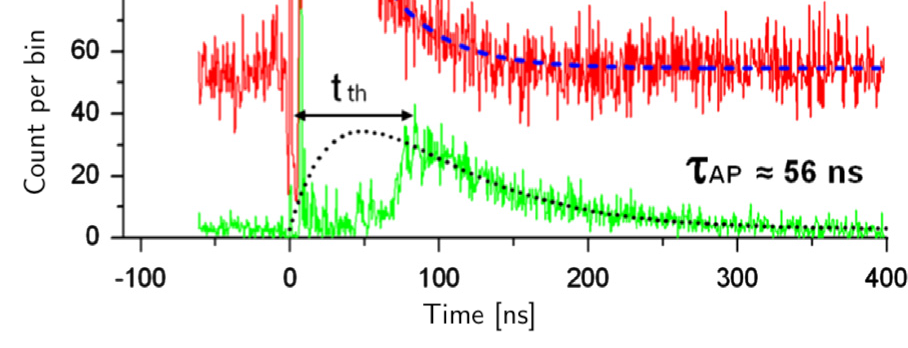
\includegraphics[width=\textwidth]{nagyap}
    
    \caption{\label{fig:nagyap} Excerpt of Figure~11 from \cite{nagy2014},
    showing the histogram of the delay of pulses successive to initial 1 PE
    pulses, selected with an upper bound on their amplitude to get afterpulses
    while removing dark count, and fitted with an exponential decay with
    constant $\tau_\text{AP}$ multiplied by the correction in
    \autoref{eq:recfactor} with $\tau_\text{rec} = \SI{207}{ns}$.}
    
\end{figure}

\cite{garutti2014} has approximately the same temporal cut and parameters, and
gets a good fit with either one or two uncorrected exponentials. We anticipate
that in our analysis the temporal cut, relative to $\tau_\text{rec}$, will be
even more extended than in the referenced articles, so we will not be able to
discriminate the two models. For simplicity, we will keep the plain
exponentials.

Another aspect to consider at small delays is the amplitude reduction. Here all
the references we consulted agree on multiplying the 1 PE amplitude by the
recharge factor \eqref{eq:recfactor}, thus assuming the amplitude to be
proportional to overvoltage. We will discuss this in relation with the results
of our data analysis.

Finally, the afterpulse avalanche itself produces trapped carriers, resulting
in multiple afterpulses. However, since it may have smaller amplitude than a
primary avalanche, we expect it to produce fewer carriers than a complete
discharge. Other two possible effects that we hypothesize, although we are not
sure about them, are: that if traps are not too far from saturation after an
avalanche, the additional afterpulses will be even more suppressed, and that an
avalanche may partially ``purge'' traps.

\stracka{Check ultima frase con Eugenio}

Keeping into account all these interactions is tedious, so we make a
simplifying assumption, inspired by the last consideration: that each avalanche
resets the cell to a fixed state. In this model, a pulse can have at most one
afterpulse. An eventual successive afterpulse must be produced by the first
afterpulse, not the initial pulse. \cite{cova1991} implicitly consider this not
to be the case, since in their statistical analysis they keep into account the
possibility of multiple afterpulses related to the same initial population of
trapped carriers. Since these are second order effects, we anticipate that the
probabilities involved are small and that we probably would not be able to
falsify the simplified model with our data.

\stracka{Eliminare ``inspired by the last consideration'' e ``since these...
our data''}

Bringing the DiCT model into the picture, each afterpulse will have its own
DiCT tree. We suppose that a smaller avalanche should emit less photons and
thus have less cross talk; again, for the sake of simplicity, we will assume
that the DiCT probability remains the same instead.

Since the DiCT involves separate cells, even with our ``resetting afterpulse''
model if the initial pulse has more than one PE then multiple afterpulses due
to the same initial pulse are allowed. In the following we refer to this case
as \emph{parallel afterpulses}, while the case with an afterpulse of an
afterpulse as \emph{series afterpulses}.

\section{Data}

We characterize DCR and correlated noise for Tile~21 from the LFoundry
production. The following data files have been collected at LNGS at different
overvoltages:
%
\begin{verbatim}
LFOUNDRY/pre-production-test/TILE_21/LF_TILE21_77K_54V_65VoV_X.wav
LFOUNDRY/pre-production-test/TILE_21/LF_TILE21_77K_54V_69VoV_X.wav
LFOUNDRY/pre-production-test/TILE_21/LF_TILE21_77K_54V_73VoV_X.wav
\end{verbatim}
%
The `\texttt{X}' suffix in the file name stands for an index which goes from~1
to~10. Each file contains $\approx\num{20000}$ events, so we have \num{200000}
events per overvoltage.

The overvoltage is obtained by subtracting the first voltage from the second in
the file name and dividing by two. The first is the breakdown voltage while the
second is the applied reverse bias; the division by two is due to the SiPM
connection layout in the PDM consisting of several parallel branches each with
two SiPMs in series. Thus the overvoltages are \SI{5.5}V, \SI{7.5}V, \SI{9.5}V.

We show the time-value histograms of a single file per overvoltage in
\autoref{fig:hist2dtile21}. Looking at the histograms it can be inferred that
the laser fires at $\approx\SI9{\micro s}$. These files do not include the
laser trigger waveform, but the external trigger from the laser ensures these
waveforms are aligned within \SI{22}{ns}. Since the DAQ configuration in the
LNGS setup was not modified between the various data taking campaigns, we check
this alignment by plotting in \autoref{fig:triggerhist} the position of the
trigger rising edge from the runs in which it was recorded. The full range of
the distribution is \SI[separate-uncertainty=true]{8969 \pm 11}{Sa}.

\begin{figure}
    
    \widecenter{\includempl{figtriggerhist}}
    
    \figcaption{triggerhist}{Cumulative histogram of the trigger leading edge
    (the first sample less than 600 in the recorded waveform) for 96 LNGS
    files. The distribution has the shape of a convolution between two uniforms
    with length 16 and~8.}
    
\end{figure}

In some of the datasets for Tile~21 we observe double peaks in the fingerplot,
i.e.~there are two possible pulse amplitudes corresponding to the same number
of PE. This is particularly evident in the first file at \SI{5.5}{VoV},
\nolinkurl{LF_TILE21_77K_54V_65VoV_1.wav}. In \autoref{fig:doublepeak} we show
the fingerplot, both global and as a function of time, computed with
\SI{1.5}{\micro s} charge integration. It is evident that the pulse charge
changes during the acquisition. Since it is still possible to separate the PE
peaks, even if they are doubled, this will not be an issue. Moreover, with the
filter we will use in the analysis the doubling will be much less marked.

\stracka{Hai un plot a supporto di questo statement? \upshape Risposta: beh,
i fingerplot che ci sono dopo. Potrei farne uno apposta qui se proprio serve.}

\begin{figure}
    
    \widecenter{\includempl{figdoublepeak}}
    
    \figcaption{doublepeak}{The distribution of the mean of the waveforms from
    sample 8958 to \num{10457} (1500 samples) in the first file at
    \SI{5.5}{VoV}. Left panel: global distribution. Right panel: the same
    distribution by groups of 200 events.}
    
\end{figure}

In this data there could be a significative amount of light that hits the
detectors after being reflected. Since the apparatus is small, we
conservatively assume an upper bound of \SI{1}m for the distance traveled by
light, which corresponds to a \SI{3}{ns} delay. This delay is smaller than the
scale of the variations of the signal shape and of the noise, so we can neglect
this problem.

\section{Peak finding}

To characterize the LFoundry Tile and classify the noise pulses we measure the
amplitude and temporal position of all pulses in data. We filter the waveforms
to suppress noise and then run a peak finding algorithm. This sections
described the various steps of the signal processing.

\subsection{Filtering}
\label{sec:filtering}

\begin{figure}
    
    \widecenter{\includempl{figtemplates}}
    
    \figcaption{templates}{Templates of the pulse shape obtained with averaging
    for each file.}
    
\end{figure}

We filter each event using a cross correlation filter (see
\autoref{sec:filters}). We follow the procedure outlined in
\autoref{sec:cctemplate} to build the filter template. We determine the
template separately for each file, to check for unexpected variations in the
pulse shape. The templates obtained are shown in \autoref{fig:templates}.
Although the variations appear to be reasonably small, we use each template
only for its own file. An unexpected feature is the nonlinearity of the pulse
amplitude with overvoltage. A possible explanation is a bookkeeping mistake,
i.e., that the recorded operating operating bias voltage is wrong. We will come
back to this discussion after the analysis.

Filtering increases the signal to noise ratio, but degrades the separation
between close peaks. Since we are studying correlated pulses, it is thus
important to use a filter as short as possible. We filter the waveform with a
logarithmic range of filter lengths: \SI{32}{ns}, \SI{64}{ns}, \ldots,
\SI{2048}{ns}. The computations we will describe are carried in parallel with
all filter lengths, and then we choose in the analysis which lengths to use.
The truncation of the template to the desired length is done as explained in
\autoref{sec:cctemplate}, keeping the fixed length subrange of samples that has
maximum squared norm.

The template is normalized to unit sum for filtering, such that the
filter behaves like an average and the baseline can be computed independently
of the filter. This also means that signals will stay negative after filtering.

To evaluate the filter near the boundaries, the waveform is prolonged with the
estimated baseline value, described in the next section. We defer to
\autoref{sec:pe} the description of how we select the filter length.

\subsection{Baseline}

To compute the height of the peaks we have to subtract the baseline value. We
compute the baseline using the pre-trigger region of the waveforms. For
robustness against deviations we use the median instead of the average. Since
the input sequence is quantized with 10~bit resolution and the median can
output only one of the values of the input sequence, the median is also
quantized. To have a more continuous output we divide the array in 8
interleaved subarrays, i.e., the first subarray contains samples 0, 8, 16,
\dots, the second 1, 9, 17, etc., take the median separately on each subarray,
and then average the medians. If any pre-trigger sample in an event is less
than 700, for that event we reuse the baseline obtained in a previous event.

In \autoref{fig:baseline} we show the histogram of the obtained baseline values
for the \SI{5.5}{VoV} data. We will carry on the discussion always on the
\SI{5.5}{VoV} dataset as example, unless otherwise necessary.
Appendix~\ref{ch:analplot} contains additional plots that complete the picture.

The baseline distribution has a small tail to the left (note that the scale is
logarithmic) and some far outliers. In \autoref{fig:bsoutlier} and
\autoref{fig:bstail} we show the events corresponding to the lowest and highest
measured baselines and a pair of events from the lower tail respectively. (The
event visualization contains elements which we have not introduced yet, they
will soon be explained.)

\begin{figure}
    
    \widecenter{\includempl{figbaseline}}
    
    \figcaption{baseline}{Distribution of the waveform baseline measured in
    the pre-trigger region of the events. See \autoref{fig:baseline2} for all
    overvoltages.}
    
\end{figure}

\begin{figure}
    
    \widecenter{\includempl{figbsoutlier-0}\includempl{figbsoutlier-1}}

    \figcaption{bsoutlier}{The events with the lowest and highest baseline.
    See \autoref{fig:bsoutlier2} for all overvoltages.}

\end{figure}

\begin{figure}
    
    \widecenter{\includempl{figbstail-0}\includempl{figbstail-1}}

    \figcaption{bstail}{A pair of events from the low baseline tail (baseline
    between 955 and 956). See \autoref{fig:bstail2} for all overvoltages.}

\end{figure}

In all cases the extreme baseline events do not show anomalies, they have
genuinely unusual baselines. At \SI{5.5}{VoV} and \SI{9.5}{VoV} the events
corresponding to the lowest and highest baseline have close progressive
indices, so they must occur close in time; we suppose then that these
deviations are due to low-frequency transient oscillations.

The events in the tail all have a pre-trigger pulse (we checked only the two
ones we plotted, we did not cherrypick). This means that we will systematically
underestimate the amplitude of pre-trigger pulses. However, as is already
evident by looking at the event plots, the bias is small compared to the pulse
height. If data with lower SNR was to be processed, we would raise (recall the
signals are negative) the baseline veto value from 700 to something as close as
possible to the noise pedestal, and segment the baseline computation to detect
inhomogeneity, but in the present case this is not deemed necessary.

\subsection{Identification of the laser peak}
\label{sec:laser}

The laser pulse occurs at a fixed offset from the start of the recorded
waveform, so we search for the primary signal associated to the laser light
emission in a range of \SI{\pm 30} samples around the expected position after
filtering. When using different filters, we adjust the search window to account
for the offset introduced by the filtering procedure. In this window we take
the minimum local minimum, i.e., we consider the samples which have higher
neighboring samples, and take the minimum of these. If there is no local
minimum, which happens when the waveform is monotonically increasing or
decreasing within the 60 selected samples, we mark the laser peak as missing.

\begin{figure}

    \widecenter{\includempl{figlaserpos-0}\includempl{figlaserpos-1}}

    \figcaption{laserpos}{Left panel: histogram of the laser peak position,
    only for 1 PE peaks, for all filter lengths. The zero of the scale is such
    that the expected position is 8969. Right panel: 2D histogram of the laser
    peak position and the amplitude, for the same selection of peaks, but only
    with the \SI{128}{ns} filter. See \autoref{fig:laserpos2} for all
    overvoltages.}
    
\end{figure}

\stracka{Hai due spiegazioni alternative: quale sarebbe l'impatto sulla tua
analisi nei due casi? (ossia, quanto ce ne frega di questa cosa?) Cosa succede
se cambi la finestra di ricerca di questo picco? \upshape Risposta: ce ne frega
poco perché non pigliamo gli afterpulse entro 30 ns di sicuro, infatti avevo
scritto ``giusto per essere controllare'' ma me l'hai fatto cancellare, uno
controlla le cose sospette perché magari scopre problemi più ampi. La finestra
l'ho cambiata durante il lavoro da \num{\pm 80} se ricordo bene a quella
attuale \num{\pm 30}, i risultati sono robusti, però non ho salvato queste cose
per bene. Potrei aggiungere alla fine del capitolo una considerazione che ho
cambiato varie cose (template, parametri vari) e i risultati sono cambiati meno
dei loro errori, eccezion fatta per il minimo delay a cui piglio gli afterpulse
che si vede l'effetto ma credo comunque entro gli errori, non ricordo bene
perché poi sono passato a 2 tau.}

As a crosscheck for this procedure we look at the distribution of the peak
positions for \SI1{PE} pulses (\autoref{fig:laserpos}, left panel). We select
\SI1{PE} pulses with a cut on the pulse height, described later in
\autoref{sec:pe}. The distribution is centered in the expected place. However,
it has a tail to the right when the filter length is short. A possible
explanation could be that when the SNR is not high enough, the peak finder
sometimes selects a close afterpulse instead of the primary pulse. Another
possible interpretation is that this tail is due to random fluctuations.

\stracka{Non andare a capo}

As a first diagnostic, we look at the joint distribution of the
peak position and height (\autoref{fig:laserpos}, right panel). If the minimum
were moving to the right due to an additional close peak, we would expect a
positive correlation between height and position in the tail. Instead, we see a
negative correlation.

\stracka{perché ce l'aspettiamo? non sono convinto \upshape Risposta: te lo
spiego, mo' non ho tempo di scriverlo, sono lentissimo a scrivere}

Then we look at the events themselves. In \autoref{fig:lptail} we show an event
in the tail at \SI{64}{ns}, filtered with \SI{64}{ns} and \SI{128}{ns}. With
the longer filter the position goes back to the center of the distribution. We
inspected a lot of events in the tail and they are almost all like the one we
show.

\begin{figure}

    \widecenter{\includempl{figlptail-0}\includempl{figlptail-1}}

    \figcaption{lptail}{Left panel: an event with unusually late laser peak
    position for 1 PE peaks with filter length \SI{64}{ns}. Right panel: the
    same event with filter length \SI{128}{ns}. See \autoref{fig:lptail2} for
    all overvoltages.}

\end{figure}

\stracka{questo va accompagnato da un commento su come cambiano i template tra
i diversi OV. come cambia l'esponenziale all'aumentare dell'OV? Es. Fig. 7.18
\upshape Risposta: secondo me non c'entra, o meglio cambiano molto poco, non
mi sembra nemmeno il caso di menzionarlo.}

Finally, the tail contracts as the overvoltage increases (see
\autoref{fig:laserpos2}). From these observations we induce that the right
shift is caused by random fluctuation. The asymmetry of the tail reflects the
asymmetry of the shape of the signal.

We said that with our procedure a laser peak can be missing. However we know
that the laser is always present; even when there are no pulses, we need to
count the event as a 0 PE laser signal to fit the Poisson+DiCT distributions.

\stracka{A possible issue can arise when some filters identify a primary pulse
from the laser, while other filters do not. \upshape Risposta: questa frase non
mi sembra sensata, ho cambiato un po' la spiegazione, vedi se capisci.}

First, we count these ``missing laser'' events for each filter length
(\autoref{fig:missing}, left panel). They are about \SI{1.5}\% of the total
number of events in the dataset, \num{200000}, so not negligible. We went
through a lot of these events and they are almost all genuinely missing pulses.
It turns out that the noise is actually quite likely not to produce a local
minimum in a \SI{60}{ns} window after filtering. Nevertheless, there are some
events which have a pulse which for some weird combination of noise
oscillations is not detected properly.

\begin{figure}

    \widecenter{\includempl{figmissing}}
    
    \figcaption{missing}{Left panel: for each overvoltage, the fraction of
    events where there is no local minimum in the laser peak search range, as a
    function of filter length. Right panel: the fraction of events where the
    minimum is missing for all filter lengths less than or equal to the one on
    the abscissa.}

\end{figure}

As in the case of the position distribution tail, the anomalies tend to appear
only for a particular filter length choice and disappear on the same event with
other lengths. So as a simple solution we use the shortest filter which yields
a non-missing peak when the preferred filter does not work. The right panel of
\autoref{fig:missing} shows how the fraction of missing events decreases as we
allow more lengths to choose from. Even with this fix, however, there is a hard
core of events which do not have a local minimum in any case, about \SI{0.15}\%.

These events are more interesting, so we show 12 of them at random for each
overvoltage in Figures~\ref{fig:verymissing0}, \ref{fig:verymissing1},
and~\ref{fig:verymissing2}. By eye we identify three cases: 1)~true missing
pulses, 2)~delayed pulses which fall out of the window, and 3)~pulses which are
shadowed by a very high close consecutive pulse. In \autoref{tab:missing} we
list the total number of hard misses and the counts of the three categories in
the sample for all overvoltages.

\begin{table}
    
    \widecenter{
        \begin{tabular}{S[table-format=1.1] S[table-format=3] *3S[table-format=1]}
            \toprule
            & & \multicolumn3c{Count of 12} \\
            \cmidrule(l){3-5}
            {Overvoltage [\si{V}]} & {Total} & {True miss} & {Delayed} & {Close consecutive} \\
            \midrule
            5.5 & 253 & 10 & 1 & 1 \\
            7.5 & 190 &  7 & 3 & 2 \\
            9.5 & 324 &  7 & 2 & 3 \\
            \bottomrule
        \end{tabular}
    }
    
    \tabcaption{missing}{The number of events where the laser peak is missing
    with all filter lengths, and the counts, in a random sample of 12 of these
    events, for the three categories of configurations that appear in this
    selection.}
    
\end{table}

\stracka{Eliminare questo paragrafo \upshape Risposta: perché? Perché non siamo
sicuri? Mi sembra meglio dirlo e dire che non siamo sicuri che stare zitti.}

The delayed pulses could be photons that produce carriers in an inactive region
that then migrate to a diode junction (we are not sure about this, it is just
speculation). The consecutive pulses could be DeCT with high DiCT, they would
have the time scale we expect from \cite[fig.~3.8~p.~54]{savarese2018} already
mentioned in \autoref{sec:sipmnoise}, or less likely afterpulses.

Since these events are a small fraction of the sample we did not investigate
this further. We will just keep in the back of our minds that there are these
events and check case by case that ignoring them has a negligible effect.

\subsection{Identification of secondary peaks and peaks not associated to the
laser pulse}

We identify other pulses using a prominence-based peak finder. In this section
we describe the peak-finding algorithm as applied to positive pulses
(low-to-high-to-low). By changing the sign of the input, the same algorithm can
be used to find minima, i.e., peaks corresponding to negative signals.

The topographical prominence is defined as follows: starting from the peak
whose prominence is to be measured, go to the right and to the left until an
higher elevation is found. For each side, take the minima between these stops
and the peak. The prominence is the difference in elevation between the peak
and the maximum of the two minima. See \autoref{fig:prominence} for an
illustration.

\begin{figure}
    
    \widecenter{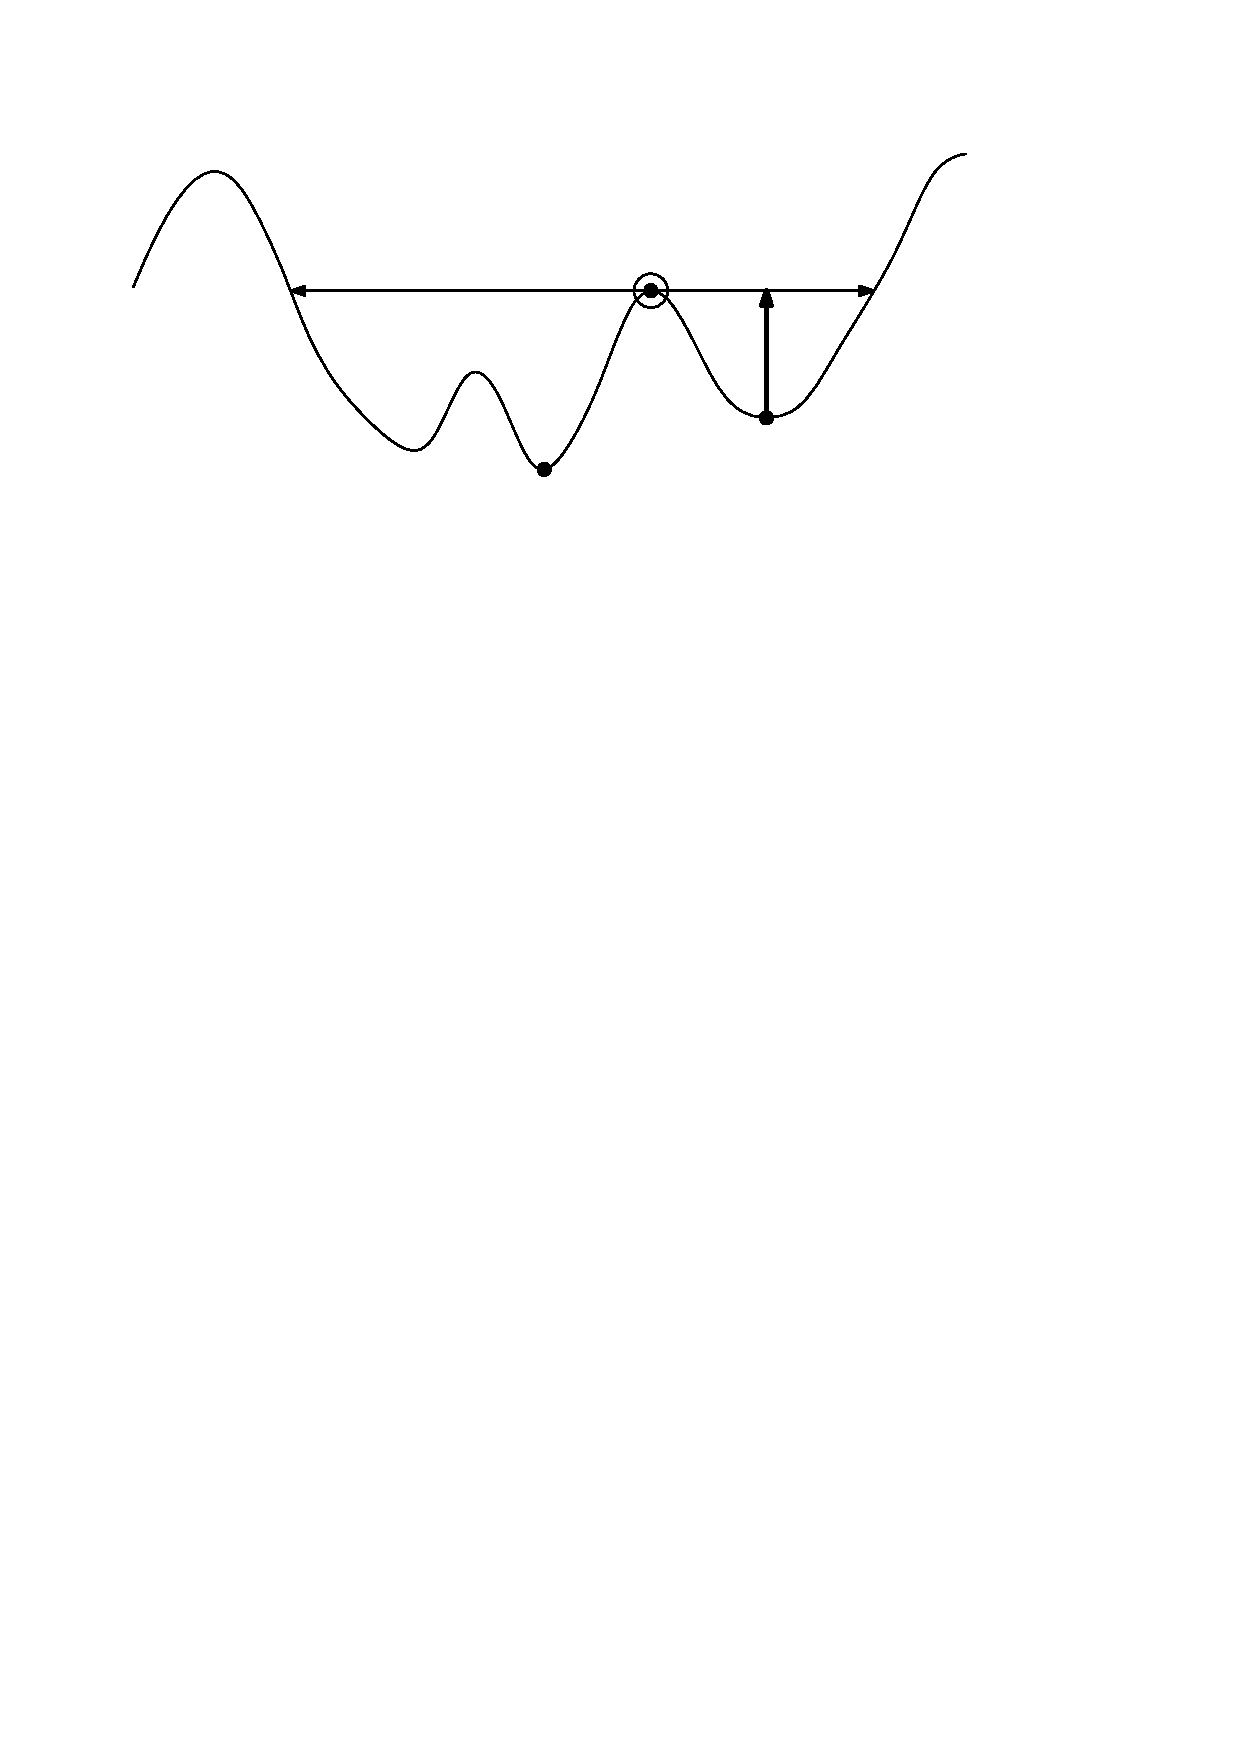
\includegraphics[width=0.8\textwidth]{prominence}}
    
    \caption{\label{fig:prominence} Illustration of the definition of
    topographical prominence. The prominence of the circled peak is the length
    of the thick vertical arrow.}
    
\end{figure}

We search the non-laser pulses separately in the pre- and post-laser peak
regions. We use the position of the laser peak, when present, to delimit the
two regions. This means that even if the laser peak is lower than the peak, the
prominence ``exploration range'' stops there. When the laser peak is missing,
we use the left edge of the laser peak search window as delimiter.

If one of the minima occurs at the edge, it is ignored and the prominence is
computed using the minimum on the other side, unless both minima occur at the
edge. This is to avoid assigning a very low prominence to a pulse whose shape
is truncated due to being close to a boundary.

The minima are capped to the baseline: if a minimum is lower than the baseline,
the value of the baseline is used instead to compute the prominence. This
increases the ratio between the prominence of close pulses to the one of
isolated pulses, because if the explored range is longer it is easier to find a
deeper random oscillation.

For each region, we save the two most prominent peaks. We do not apply a
threshold on the prominence, we always fill the four slots per event. In this
way we can observe the distribution of the height of random peaks and choose a
good threshold afterwards.

\marginpar{A Stracka: qua mi hai chiesto di spostare le cose, ma non ho capito
bene come}

In peak finding algorithms it is customary to require a minimum distance
between peaks. This is to avoid picking up close high peaks due to random
oscillation that actually correspond to a single pulse. Selecting by prominence
avoids this problem if the waveform is smooth, because close peaks will have
only a shallow dip between them and the prominence of the lower one will be
measured relative to that, resulting in a very low prominence. Our waveforms
are smooth on the scale of the filter length, so it did not turn out necessary
to add a distance criterion.

In \autoref{fig:peakfinder} we show two examples of events with close pulses
correctly identified.

\begin{figure}
    
    \widecenter{\includempl{figpeakfinder-0}\includempl{figpeakfinder-1}}
    
    \figcaption{peakfinder}{The events with the closest pair of pre-trigger
    pulses (left panel) and post-trigger pulse closest to the laser pulse
    (right panel) for at least 1 PE peaks.}
    
\end{figure}

\subsection{Number of photoelectrons associated to a peak}
\label{sec:pe}

To assign the number of PE to the peaks we need to define bins for the height
of the peaks. We want to choose the filter length that yields the optimal
separation between PE in the height distribution. A longer filter suppresses
the random height fluctuation due to noise; at the same time, however, it picks
up afterpulses with the template tail, adding an upper tail to each PE height
distribution. Since the afterpulse probability increases with the number of PE
of the primary pulse, the distributions for 0 and 1~PE are the least affected.

In our analysis we will care particularly about selecting 1~PE pulses and
separating the afterpulses. So we use the following criterion: we take the
shortest filter that allows to clearly separate the 1~PE distribution. These
filter lengths are respectively \SI{128}{ns}, \SI{64}{ns}, \SI{64}{ns} for
\SI{5.5}{VoV}, \SI{7.5}{VoV}, \SI{9.5}{VoV}. We show the templates for these
lengths in \autoref{fig:trunc}.

\begin{figure}

    \widecenter{\includempl{figtrunc}}
    
    \figcaption{trunc}{The principal filter templates used in the analysis,
    shown unnormalized.}
    
\end{figure}

We tried selecting away the afterpulse tails using the peak finder to locate
afterpulses, however we did not manage to reduce them significantly. We
interpret this as the tail being composed mainly of afterpulses occurring
shortly after the primary peak, that can not be recognized individually due to
their low height. Being located on the slope of the laser peak, the prominence
of a close afterpulse tends to be lower than that of an isolated pulse with the
same height. For close enough afterpulses, the prominence will often be lower
than noise fluctuations, and the peak finder will fail in identifying them.

There are other two minor factors that deform the height distribution: the
saturation of the digitizer, and the tails of pre-trigger pulses close to the
laser one. Thus we histogram the laser peak height excluding events with
saturation and events where the peak finder locates a pre-trigger pulse higher
than the upper endpoint of the random peaks height distribution within
\SI{2.5}{\micro s} before the trigger using the longest filter. This histogram
is shown in \autoref{fig:pe} for \SI{5.5}{VoV} and \autoref{fig:pe2} for all
overvoltages.

\begin{figure}
    
    \widecenter{\includempl{figpe}}
    
    \figcaption{pe}{Histogram of the laser peak height, with a selection to
    avoid biased heights. The dotted lines are the boundaries of the PE bins.
    See \autoref{fig:pe2} for all overvoltages.}
    
\end{figure}

\marginpar{Qua mi hai chiesto di cancellare delle cose, ma le lascio perché
secondo me non hai capito.}

We define the PE bin boundaries in \autoref{fig:pe} taking the midpoints
between the two most distant consecutive heights in the range between each pair
of consecutive height distribution peaks. Laser peak heights above the last
boundary are assigned to an overflow bin when necessary. The ruler ticks that
accompany the peaks in the event visualizations are these boundaries.

\stracka{eliminare ``the ruler... boundaries''}

Note the dips between the peaks in the histograms (the vertical scale is
logarithmic). The lowest bin count is at most~4 in all cases. Let us put a
rough upper bound on the contamination. This allows us to place a rough upper
bound of \SI1\% on the bin-to-bin contamination. This in particular is surely
less than the Poisson error on the count for each PE. The 1~PE peaks are well
separated, with a row of 0 or 1~count bins around them, so we estimate a
contamination of \SI{0.01}\%.

\subsection{Determination of the amplitude of close pulses}

When two pulses are close to each other, the height contains a contribution
from the tail of the other pulse. We need to compute the amplitude of the
single pulse, i.e., the height it would have if it was isolated. To simplify
the problem, we make the following assumptions:
%
\begin{enumerate}
    
    \item the position of a peak does not depend on the presence of other
    pulses;
    
    \item the shape of afterpulses is the same as normal pulses.
    
\end{enumerate}

About the first assumption: we have seen that the peaks in the output of the
cross correlation filter have a sharp cusp. A perfectly sharp cusp, even if
summed to a sloping shape, remains in the same position. A rounded peak,
instead, will move slightly in the uphill direction when summed to a slope.
Given the short filters we are using, these cusps are not really sharp, as
shown in the right panel of \autoref{fig:peakfinder}: the peak in the square
box has a radius of less than \SI{10}{ns}. Thus we estimate the typical bias
due to an underlying exponential tail to be around \SI{5}{ns}.

The second assumption is commonly made in the literature. But it rests on the
assumption that the pulse shape does not change with overvoltage, such that for
an avalanche occurring while the cell is recharging, only the overall amplitude
of the pulse will be affected. \autoref{fig:shape} shows that while the shape
of the signal pulses varies with overvoltage for the Tile under study, the
difference is small enough to justify the working hypothesis.

\begin{figure}
    
    \widecenter{\includempl{figshape}}

    \figcaption{shape}{The signal templates at different overvoltages compared
    fixing the peak amplitude to~1. The thickness of the stroke is twice the
    standard deviation over the 10 files per overvoltage, while the center of
    the stroke is the mean.}
    
\end{figure}

Now, let $\mathbf y$ be the output of the filter applied to a single noiseless
pulse, which we compute by filtering the signal template. Let $t_\alpha$ be the
position of peak $\alpha$ and $a_\alpha$ the unknown amplitude. Since the
filter is linear, the filtered sum of the pulses and the noise is the sum of
each component filtered separately, so the model for the complete filtered
waveform $\mathbf w$ is
%
\begin{equation}
    w_i = \sum_\alpha a_\alpha y_{i - t_\alpha} + \epsilon_i,
\end{equation}
%
where $\boldsymbol\epsilon$ is the filtered noise. There is some freedom in the
definition of $\mathbf y$: we fix that the peak occurs at $y_0$ and that $y_0 =
1$, such that if there is only one peak then $w_{t_1} = a_1 + \epsilon_{t_1}$.

It is well known that the minimum variance in estimating $\mathbf a$ is
obtained by using least squares with the inverse of the covariance matrix $V$
of $\boldsymbol\epsilon$ as quadratic form. Let $H_{i\alpha} = y_{i-t_\alpha}$,
then the solution is \cite[628]{zyla2020}
%
\begin{equation}
    \hat{\mathbf a} = (H^\top V^{-1} H)^{-1} H^T V^{-1} \mathbf w.
    \label{eq:lsq}
\end{equation}
%
We note, however, that to solve the system it is just necessary to have as many
datapoints as the number of peaks. It then comes natural to solve for
simplicity this system of equations instead:
%
\begin{equation}
    w_{t_\beta} = \sum_\alpha \hat a_\alpha y_{t_\beta - t_\alpha},
    \label{eq:amplsystem}
\end{equation}
%
i.e., we use only the observed peak heights $w_{t_\beta}$ instead of the full
waveform.

To justify this simplification, we recall that in \autoref{sec:filters} we said
that the matched filter is equivalent to linear least squares. We now indeed
show that, if we were using the matched filter, solving \eqref{eq:amplsystem}
would be equivalent to least squares and thus optimal. Just for this proof, let
us use all the above notation, but without the filter applied, i.e., $\mathbf
w$ is the unfiltered waveform, $\mathbf y$ is the unfiltered signal, $V$ is the
covariance of the unfiltered noise.

The model (noise implicit) is
%
\begin{equation}
    \mathbf w = H \mathbf a. \label{eq:modelni}
\end{equation}
%
The filter is applied by operating with the matrix
%
\begin{equation}
    F_{ij} \equiv V^{-1}_{jk} y_{k-i}. \label{eq:filterf}
\end{equation}
%
Here we can not write the filter as the cross correlation with a fixed template
because we are not assuming the stationarity of the noise. If that was the
case, $V^{-1}$ would be invariant under the paired translation of its indices,
and thus \eqref{eq:filterf} could be expressed with a template, and would
depend only on $j-i$. In other words, think that the template changes at each
point due to the different noise spectrum. Applying the filter to
\eqref{eq:modelni} we have
%
\begin{align}
    F \mathbf w &= F H \mathbf a. \label{eq:noindices}
\end{align}
%
We want to use only the peak heights in the filter output, assuming that we
know exactly the true signal positions. These are
%
\begin{equation}
    W_\beta \equiv (F \mathbf w)_{t_\beta} = V^{-1}_{jk} y_{k-t_\beta} w_j,
\end{equation}
%
which in vector form becomes
%
\begin{equation}
    \mathbf W = H^\top V^{-1} \mathbf w.
\end{equation}
%
So, considering only the $W_\beta$ on the left hand side of
\eqref{eq:noindices} and putting the indices on the right hand side, we have
%
\begin{align}
    W_\beta &= V^{-1}_{jk} y_{k-t_\beta} H_{j\alpha} a_\alpha = \\
    &= (H^\top V^{-1} H)_{\beta\alpha} a_\alpha,
\end{align}
%
thus the solution is
%
\begin{equation}
    \mathbf a = (H^\top V^{-1} H)^{-1} H^\top V^{-1} \mathbf w,
\end{equation}
%
which is the least squares estimator \eqref{eq:lsq}. \hfill $\square$

Our filter differs in two ways from the matched filter: it does not keep into
account the noise correlation, and it is truncated. So our method for computing
the amplitude is worse than the optimal one as much as the filter is worse than
the matched filter.

In each event we have to decide which peaks to input in \eqref{eq:amplsystem}.
Most of the time, peaks are random noise oscillation. If the amplitude of
random peaks had mean zero, adding a fake peak would increase the error but not
introduce a bias. But, since we are selecting peaks by highest prominence, it
is guaranteed that in a region of some microseconds we will find a peak with
height comparable to the noise standard deviation. Indeed in the next section
we will look at the height distribution for the peak finder output and see that
it is positively biased. So we compute the amplitude only for peaks higher than
a threshold. As threshold we pick the PE bin boundary between 0 and 1~PE.

\stracka{si capisce poco il perché della definizione di questa nuova variabile,
ma una volta che l'hai costruita come verifichi che faccia quello che vuoi che
faccia? \upshape Risposta: invece è importante! Se capisci poi non fai la
domanda su come si verifica. Se non la definisco così spariscono tutte le
strisciate di rumore dai grafici, che però esistono e semplicemente non le
starei guardando, sarebbe una finta pulizia.}

When we use the computed pulse amplitude instead of the peak height, we would
like to also see the distribution of the fake peaks such that we can be sure at
a glance that we have no contamination, but most of the fake peaks do not have
an amplitude since they do not pass the threshold prerequisite. The $y$
normalization we have chosen makes the amplitude ``have the same units'' of the
height, so we construct a variable which is the amplitude when available, and
the height otherwise. In the following sections we mean this variable when we
talk about ``amplitude''.

Note that with this selection we are not excluding low height afterpulses from
the amplitude computation, because even if their amplitude is smaller, sitting
on the tail of their parent pulse their height from baseline is still above
threshold.

\stracka{Eliminare ``in the event visualizations...'' \upshape Risposta: ci
sarebbero troppe cose da scrivere in troppe caption, per questo dico ogni cosa
una sola volta nel punto in cui la definisco.}

In the event visualizations, the ruler associated to each peak starts from a
dot placed such that the distance from the dot to the peak is the amplitude.
In the legend, the amplitude is given under ``$a = \ldots$''.

We checked that recomputing the PE bins with the laser pulse amplitude instead
of the height gives almost the same result. In the analysis, anyway, we use the
bins computed with the amplitude for complete consistency.

\section{Random pulses rate}
\label{sec:random}

When counting afterpulses there will be a background from the dark count rate,
which we have to subtract, so we measure it in the pre-trigger region. The
laser trigger frequency should be less than \SI{1}{kHz}, so the events are
distant between each other and there is not the possibility of correlated noise
from a laser pulse leaking into the successive event.

\marginpar{What is the laser trigger rate? Specify this better if I know after
writing \autoref{ch:data}.}

The title of this section reads ``random pulses rate'' instead of dark count
rate because we will see we have reason to believe that in the data there are
actually more random pulses than the dark count. It does not matter for
background subtraction though.

By looking at the time-value histograms in \autoref{fig:hist2dtile21} we see
that in \num{20000} events there are just a few pre-trigger pulses, so we
neglect the case of a double random pulse in the same event. If there are two
pre-trigger pulses, one must be the afterpulse of the other, so the event
counts as one random pulse. For the rate we do not care to know which pulse is
the primary, but we will need it when fitting the DiCT model to the random
pulses.

The primary pulse is of course the first in chronological order, but to
distinguish the one pulse from the two pulses case we are forced to put a
threshold on the amplitude before looking at the distribution. We do something
similar as we did for the amplitude. The initial variables are the position,
height and amplitude of the two most prominent pre-trigger peaks. When both
heights are above the 0 to 1~PE boundary, the first set of variables is set to
the first peak in chronological order; otherwise to the most prominent peak.

In the left panel of \autoref{fig:pretrigger} we show the scatter plot of the
first pulse amplitude versus position. There are some problems at the edges. On
the left edge, the negative amplitudes are actually very large values that we
mapped to \num{-10}. They are probably due to the amplitude linear system
\eqref{eq:amplsystem} being degenerate, but we did not investigate why this may
happen. On the right edge conversely there are some zeroes and anomalously
small values. Thus we ignore the first \SI{100}{ns} and the last \SI{500}{ns}
of the pre-trigger region. The wider margin on the right is just to be safe in
case the presence of the laser pulse was having some effects. The selected
region is marked by the gray vertical band in the plot.

\begin{figure}
    
    \widecenter{\includempl{figpretrigger-0}\includempl{figpretrigger-1}}
    
    \figcaption{pretrigger}{Left panel: scatter plot amplitude vs.\ position of
    the chronological first pre-trigger peak in each event. Right panel:
    histogram of the amplitude for the peaks contained in the vertical gray
    band in the left plot. See \autoref{fig:pretrigger2} for all overvoltages.}
    
\end{figure}

The right panel of \autoref{fig:pretrigger} shows the histogram of the
amplitude of the pulses in the temporal cut. The separation between random
peaks and 1~PE pulses is clear; the amplitude threshold we use is marked with a
gray band also reported in the left panel. The dotted lines are the PE bin
boundaries. As we anticipated, the distribution of the amplitude of the random
peaks is biased upward, and leaks a bit above the 0 to 1~PE boundary.

To compute the rate, we count the number of pulses satisfying the cuts, and
divide by the number of events times the pre-trigger region duration minus the
cuts. The uncertainty is given by the Poisson error of the count. In
\autoref{tab:ptrate} we report the obtained values.

\begin{table}
    
    \widecenter{
        \raisebox{-0.5\height}{\includempl{figptrate}}
        \begin{tabular}{
            S[table-format=1.1]
            S[table-format=6]
            S[table-format=1.2]
            S[table-format=1.2]
            S[table-format=3]
            S[table-format=3(2), separate-uncertainty=true]
        }
            \toprule
            &
            & \multicolumn2c{Time}
            & \multicolumn2c{Pulses} \\
            \cmidrule(lr){3-4} \cmidrule(l){5-6}
            {Overvoltage}
            & {Events}
            & {Per event}
            & {Total}
            & {Count}
            & {Rate} \\
            {[\si V]}
            &
            & {[\si{\micro s}]}
            & {[\si s]}
            &
            & {[\si{cps}]} \\
            \midrule
            5.5 & 200028 & 8.37 & 1.67 &  73 &   44 \pm 5 \\
            7.5 & 200021 & 8.37 & 1.67 & 277 & 165 \pm 10 \\
            9.5 & 200025 & 8.37 & 1.67 & 186 &  111 \pm 8 \\
            \bottomrule
        \end{tabular}
    }
    
    \tabcaption{ptrate}{The rate of primary pre-trigger pulses in a fiducial
    region and the intermediate quantities used to compute it.}
    
\end{table}

We notice that the rate at \SI{7.5}{VoV} is substantially higher than the one
at \SI{9.5}{VoV}. The dark count rate steadily increases with overvoltage (see
for example \cite[fig.~3.13~p.~61]{savarese2018}), because an higher field in
the diode lowers the potential barrier that a carrier must overcome to become
conducive. So we induce that there must be an additional source of random
pulses. Maybe the experimental setup was not light-tight. Anyway, these values
can be considered an upper bound for the dark count rate. For reference, the
maximum dark count rate allowed by the DarkSide20k specifications is
\SI{250}{cps} \cite[tab.~3.1~p.~62]{savarese2018}.

\section{Afterpulses}

To study afterpulses we consider the post-trigger peaks in events with a 1~PE
laser pulse. Using the terminology introduced at the end of
\autoref{sec:aptheory}, a single PE initial pulse implies that there are no
parallel afterpulses. The parameter we are interested in is the probability for
a single cell to generate an afterpulse, thus even if there are two series
afterpulses, we only care about the first. So, like we did for pre-trigger
peaks, when there are two peaks with height above the 0 to 1~PE boundary we
select the first.

The case with an afterpulse and a random pulse is quite unlikely. From
\autoref{tab:ptrate} we compute that the probability of having a random pulse
in the post-trigger region is within \SI{0.1}\%. We will see that the
probability of an afterpulse is about \SI{5}\%, so the coincidence probability
is less than \SI{0.005}\%, in less than \num{50000} events, so we expect less
than 2.5 afterpulse+random events. Since the distribution of randoms is flat,
while the afterpulses are concentrated at short delays, and keeping into
account that even if both were uniform in half of the cases the afterpulse
would come first by chance, we are sure that the expected afterpulses lost due
to random are less than 1 and so we neglect this problem.

The amplitude of the afterpulses is shorter than normal at low delays. It would
be convenient to select them with a straight cut. This will be even more useful
when fitting the DiCT model on the afterpulses. We empirically observe that the
height of the afterpulses is approximately constant, although a bit higher at
short delays, like if the rule was that an afterpulse reaches a normal height
when ``sitting'' on the tail of its parent (see the top right panel of
\autoref{fig:apampl}). The slight increase for close pulses can be interpreted
as an effect of the smearing of the filter. So we do the following: we take the
\emph{unfiltered} signal template, normalize it to have peak amplitude as a
1~PE \emph{filtered} pulse, take its value at a delay from its peak equal to
the delay from the post-trigger to the laser peak, and sum this to the
post-trigger pulse amplitude.

\begin{figure}
    
    \widecenter{\includempl{figapampl-0}\includempl{figapampl-1}}

    \widecenter{\includempl{figapampl-2}\includempl{figapampl-3}}
    
    \figcaption{apampl}{Various ways of measuring the magnitude of post-trigger
    pulses. Top left: the prominence computed by the peak finder; it decreases
    with short delays so it does not allow a straight cut. Top right: the
    height from the baseline; it is straighter but leaks a bit above the 2~PE
    threshold. Bottom left: the amplitude; it yields a better separation than
    the prominence but has to be rectified. Bottom right: the corrected
    amplitude which we use in our analysis.}
    
\end{figure}

The obtained \emph{corrected amplitude} is shown in the bottom right panel of
\autoref{fig:apampl}. Note that this correction is not equivalent to dividing
by the expected recharge factor \eqref{eq:recfactor}, it is just an empirical
procedure that rectifies the observed distribution. This may indicate that the
model is inaccurate, however we did not investigate further. In the event
visualizations, the amplitude shown for post-trigger pulses is actually the
corrected amplitude.

We can now discuss an additional issue with selecting the first peak when there
are two of them. Before computing the amplitude we select by height. Pulses
sitting on the tail of the laser pulse have a height bonus, and we said this is
useful to avoid selecting away short afterpulses at this stage. However some of
these short pulses will turn out to be noise. If it happens that there is a
second true pulse, it will be hidden by the first noise pulse. So we take the
first chronological only when both have their corrected amplitude above the 0
to 1~PE threshold. We checked that at \SI{5.5}{VoV} there would be at most 13
cases with this problem, to be compared to about 500 selected post-trigger
pulses, so the effect would be small anyway.

To select the afterpulses we have to ignore short delays because we can not
separate too short pulses from the noise, and because the peak finder could be
losing some pulses if they are short and close to the laser peak. Moreover,
like with the random pulses, the threshold on the corrected amplitude has to be
set higher that the 1~PE boundary because the amount of noise is overwhelming
compared to the pulses. We also truncate the delay distribution at
approximately \SI{500}{ns} from the end of the waveform just to stay safe from
boundary effects. We first do the temporal selection, and then determine the
threshold with our usual procedure of taking the midpoint between the two most
distant consecutive samples. These selections are shown in
\autoref{fig:apscatter}.

\begin{figure}
    
    \widecenter{\includempl{figapscatter-0}\includempl{figapscatter-1}}

    \figcaption{apscatter}{Left panel: corrected amplitude versus delay from
    laser peak; the gray bands mark the selected ranges. Right panel: the
    histogram of the amplitude for the points that fall in the vertical band in
    the scatterplot. See \autoref{fig:apscatter2} for all overvoltages
    and a zoom in of the scatterplot.}
    
\end{figure}

We have done a temporal cut, thus to count the afterpulses we have to calculate
how many we have lost. To do this we need to determine the temporal
distribution and compute the probability mass that falls outside of the
selected range. We histogram the delay of the pulses and fit two distributions,
one with an exponential decay component and one with two.

Since we are selecting the first pulse after the laser peak, normally it would
be necessary to correct the distribution for a ``first arrived'' effect: an
eventual second pulse would not be counted, so the observed counts decay faster
with delay than the actual distribution. Simple example: start from a uniform
distribution, and take the first event after a fixed point in time; the
distribution transforms into the well known exponential. \cite[2]{cova1991} and
\cite[4]{garutti2014} both take this into account. In our case, however, we
have a model where caring only about the first pulse is ``built-in'' so to say.
Just for reference, asymptotically the correction would amount to the
probability of afterpulses, which as we will see is about \SI{5}\%.

This is not true for the background of random pulses, which would need the
correction, but its probability is so small that the correction can be
neglected. In other words: we approximate the exponential background of random
pulses with a uniform because the rate is very low compared to the observed
time interval.

We do an approximate Bayesian fit using least squares. This is described in
detail in \autoref{ch:fit}; for the impatient, just consider that this is
almost a standard least squares fit of a histogram, with additional squared
terms that represent the prior.

The priors of the fit are:
%
\begin{itemize}
    
    \item The expected uniform background, computed from the random pulse rate
    in \autoref{tab:ptrate}. The variance is determined only from the variance
    of the rate; the afterpulse count i.e., the histogram normalization is an
    errorless input.
    
    \item For the one component fit, the prior on the logarithm of the
    exponential decay constant in nanoseconds is $\log(1000) \pm 1$. Consider
    than a $\pm 1$ error on the natural logarithm corresponds to a \SI{100}\%
    relative error with first order propagation.
    
    \item For the two components fit, the priors on the logarithms are
    $\log(400) \pm 1$, $\log(800) \pm 1$, while the prior on the relative
    weight of the short component is a uniform in $(0, 1)$.
    
\end{itemize}

All the parameters are bounded, so they are fit transformed. The background
density and the exponential scales are transformed with the logarithm, while
the component weight is mapped to the unitary interval using the error
function, which makes the prior on it uniform.

Since the density varies a lot over the observed range of about \SI{5}{\micro
s}, we use uneven bins for the fit. As simple criterion we compute the bins
that would yield uniform counts with an exponential with scale \SI{1.5}{\micro
s}:
%
\begin{equation}
    b_i = t_L - \tau_0 \log\left(1 - \frac in
    \left(1 - \exp\left(-\frac{t_R - t_L}{\tau_0}\right)\right)\right),
    \quad i = 0, \ldots, n,
\end{equation}
%
where there are $n$ bins, $b_i$ is the $i$-th bin edge, $\tau_0 =
\SI{1.5}{\micro s}$, and $(t_L, t_R)$ is the total range. For $n$ we take 3/4
of the square root of the total count. With these criteria it never happened
to have a bin with a count less than~5.

We are using somewhat large bins, so we have to fit against the integral of the
distribution instead of the usual approximation of taking the density in the
center of the bin. The cumulative density functions for the two models are:
%
\begin{align}
    P_1(t_L < t' < t;\tau,R) &=
    \left(1-\frac RN\right)
    \left(1 - e^{-t/\tau}\right)
    + \frac RN \frac t{t_R-t_L}, \\
    %
    P_2(t_L < t' < t;\tau_1,\tau_2,p_1,R) &=
    \left(1-\frac RN\right)
    \left[p_1 \left(1 - e^{-t/\tau_1}\right)\right. \notag \\
    \phantom x &+ \left.(1 - p_1)
    \left(1 - e^{-t/\tau_2}\right) \right] \notag \\
    \phantom x &+ \frac RN \frac t{t_R-t_L},
\end{align}
%
where $\tau$, $\tau_1$ and $\tau_2$ are the exponential scales, $p_1$ is
the weight of the component with the shorter prior, $R$ is the number of
random pulses, and $N$ is the total histogram count.

Once we have the fitted parameters, we correct the afterpulse count by
subtracting the fitted background and dividing by the probability mass
contained in the range:
%
\begin{align}
    N_1 &= \frac {N-R} {\exp(-t_L/\tau) - \exp(-t_R/\tau)},
    \label{eq:n1} \\
    %
    N_2 &= \frac {N-R} {p_1 (e^{-t_L/\tau_1} - e^{-t_R/\tau_1})
    + (1-p_1) (e^{-t_L/\tau_2} - e^{-t_R/\tau_2})},
    \label{eq:n2}
\end{align}
%
then we divide by the number of events to compute the afterpulse probability.
In \autoref{fig:apfit} we show the fit, while in \autoref{tab:ap} and
\autoref{fig:apresults} we summarize the results for all overvoltages. In all
the calculations, when necessary, we have kept into account the correlations to
propagate the error.

\marginpar{It may be useful to compute the number of afterpulses weighted with
the amplitude, since the afterpulses get denser as they get shorter.}

\begin{figure}
    
    \widecenter{\includempl{figapfit-0}\includempl{figapfit-1}}

    \figcaption{apfit}{Left panel: fit of the temporal distribution of
    post-trigger pulses. Right panel: the histogram with even bins and without
    the temporal cuts. In the legend, `const' is the background excess density,
    i.e., $(R/N)/((t_R-t_L)(1-R/N))$, in \si{ns^{-1}}. See \autoref{fig:apfit2}
    for all overvoltages.}
    
\end{figure}

\begin{table}
    
    \widecenter{
        \scriptsize\sffamily
        \setlength\tabcolsep{4pt}
        \begin{tabular}{
            S[table-format=1.1]
            S[table-format=3]
            S[table-format=4]
            S[table-format=5]
            S[table-format=3]
            S[table-format=1.2]
            S[table-format=2.1(2)]
            S[table-format=2.1(2)]
            S[table-format=3(2)]
            S[table-format=1.2(2)]
            S[table-format=2.1(2)]
            S[table-format=1.3(2)]
            S[table-format=1.2(2)]
            S[table-format=3]
            S[table-format=2]
            S[table-format=1.2]
        }
            \toprule

            & \multicolumn2c{Delay range}
            & {}
            & {}
            & {}
            & {}
            & \multicolumn4c{Fit parameters}
            & {}
            & {}
            & \multicolumn3c{Fit quality} \\
            \cmidrule(lr){2-3} \cmidrule(lr){8-11} \cmidrule(l){14-16}
            {OV}
            & {tL}
            & {tR}
            & {Events}
            & {N}
            & {Time}
            & {R prior}
            & {R}
            & {tau1}
            & {tau2}
            & {p1}
            & {Correction}
            & {Prob.}
            & {chi2}
            & {dof}
            & {pvalue} \\
            {[\si V]}
            & {[\si{ns}]}
            & {[\si{ns}]}
            &
            &
            & {[\si s]}
            &
            &
            & {[\si{ns}]}
            & {[\si{\micro s}]}
            & {[\si\%]}
            &
            & {[\si\%]}
            &
            &
            & \\
            \midrule
5.5 & 250 & 5500 & 46985 &  619 & 0.25 & 10.8 \pm 1.3 & 11.8 \pm 1.2 & 396 \pm 18 &                 &              &   1.88 \pm 0.12 & 2.43 \pm 0.18 &  81 & 18 & {<1e-6} \\
5.5 & 250 & 5500 & 46985 &  619 & 0.25 & 10.8 \pm 1.3 & 10.8 \pm 1.3 & 263 \pm 25 &   1.77 \pm 0.38 & 69.3 \pm 4.6 & 1.921 \pm 0.065 & 2.49 \pm 0.13 &  14 & 18 &    0.71 \\ \midrule
7.5 & 250 & 5500 & 38400 &  704 & 0.20 & 33.4 \pm 2.0 & 35.6 \pm 2.0 & 382 \pm 17 &                 &              &   1.93 \pm 0.12 & 3.35 \pm 0.24 &  83 & 19 & {<1e-6} \\
7.5 & 250 & 5500 & 38400 &  704 & 0.20 & 33.4 \pm 2.0 & 33.5 \pm 2.0 & 263 \pm 23 &   1.92 \pm 0.49 & 71.8 \pm 4.1 & 1.964 \pm 0.066 & 3.43 \pm 0.18 &  20 & 19 &    0.38 \\ \midrule
9.5 & 150 & 5500 & 28297 & 1072 & 0.15 & 16.8 \pm 1.2 & 17.9 \pm 1.2 & 299 \pm 11 &                 &              & 1.652 \pm 0.083 & 6.15 \pm 0.36 & 187 & 24 & {<1e-6} \\
9.5 & 150 & 5500 & 28297 & 1072 & 0.15 & 16.8 \pm 1.2 & 16.9 \pm 1.2 & 142 \pm 12 & 0.957 \pm 0.084 & 57.8 \pm 3.5 & 1.785 \pm 0.045 & 6.66 \pm 0.26 &  23 & 24 &    0.55
            \\ \bottomrule
        \end{tabular}
    }
    
    \scriptcaption{tab}{tab}{ap}{Intermediate quantities and results of the
    afterpulse analysis. For each overvoltage the data is fitted either with
    one or two exponential decay components. ``Prob.'' is the afterpulse
    probability. ``Correction'' is the inverse of the denominator in
    \eqref{eq:n1} or \eqref{eq:n2}.}
    
\end{table}

\begin{figure}
    
    \widecenter{\includempl{figapresults}}

    \figcaption{apresults}{Results of the afterpulse analysis. The first panel
    gives the probability for a 1 PE pulse to generate at least one afterpulse.
    The second shows together the exponential decay constants for the one and
    two components models. The third contains the relative weight of the short
    component for the two components model.}

\end{figure}

The one component fit has poor quality, so to compute the errors on the
correction and on the afterpulse probability, we rescale the covariance matrix
of the fitted parameters dividing by the factor $\chi^2/\text{dof}$. The two
components fit seems good so we do not rescale the errors. See \autoref{ch:fit}
for details on this procedure. In \autoref{tab:ap}, the errors on the fit
parameters are not rescaled, while the errors on the parameters entering into
the calculation of ``Correction'' and ``Prob.'' are.

Even if the two models differ, the resulting corrections and thus afterpulse
probabilities are compatible with each other for each overvoltage.

% grafici per il dect: savarese p. 59, 64.

In the top left panel of \autoref{fig:apampl}, which shows the prominence
versus delay from the laser pulse of post-trigger pulses, we notice that at
short delays, less than \SI{100}{ns}, there is a dense lump of points around
the 1~PE height. These may appear as good candidates for delayed cross talk;
however, they are all without exception cases where the laser peak is delayed
with the short filter and classified as post-trigger pulse, and the event is
still selected as 1~PE laser because we use a longer filter for the selection.
This was discussed in \autoref{sec:laser}. The same goes for the lump at 2~PE,
but by inspecting the events one by one we found a single event at
\SI{9.5}{VoV} that has a good chance of being DeCT. There are about \num{30000}
selected events for that overvoltage; supposing to have missed some cases since
we inspected by hand, we give this rough estimate: $10/\num{30000} =
\SI{0.03}\%$. The event we are talking about is shown in
\autoref{fig:dectevent}.

\begin{figure}
    
    \widecenter{\includempl{figdectevent}}
    
    \figcaption{dectevent}{An event where the post-trigger pulse appears to
    have an integer number of PE with normal amplitude (right panel) instead
    of corrected amplitude (left panel).}
    
\end{figure}

\section{Direct cross talk}

We take the random pulses and afterpulses selected in the previous sections and
the laser pulses and fit the DiCT models on the PE distributions. We assign the
pulses to the PE bins using the amplitude. For the afterpulses we use the
corrected amplitude.

Since the PE bins do not cover the full amplitude range, we put all the
uncovered pulses in an overflow bin which is fitted against the survival
function of the distribution. Saturated pulses are included.

The bins are fixed a priori independently of the effective data range, so it
does happen that there are empty bins for high PE. So for each dataset we
aggregate bins to the overflow bin starting from the last one until there are
at least 4, sometimes 5, samples in the overflow bin.

The priors for the fit parameters are: uniform in $(0,1)$ for $\mu_B$ and $p$,
and $0 \pm 1$ for $\log(\mu_P)$.

For the \SI{9.5}{VoV} laser data the overflow bin seems to be a particular
source of data-model discrepancy, so we also fit it without overflow. In this
case the bins if necessary are aggregated to the last bin. In the spirit of
avoiding arbitrary choices, we do the same at all overvoltages and also for the
afterpulses, reporting both results.

The 0~PE probability in the laser model only depends on the initial Poisson
mean $\mu_P$. Since in most of the cases the laser fit has poor quality, we are
interested in ``fixing'' the first datapoint, i.e., assuming that the Poisson
model is correct and that all the problems come from the DiCT model. As usual
we will rescale the fit errors with $\sqrt{\chi^2/\mathrm{dof}}$, so what we
want to obtain is that, after the rescaling, the error on the first datapoint
is the Poisson error. So we would like to first divide that error by what would
turn out to be the $\sqrt{\chi^2/\mathrm{dof}}$ considering the modified error.
As an approximation, we instead divide the error by the
$\sqrt{\chi^2/\mathrm{dof}}$ obtained with the normal fit.

In \autoref{fig:ctfitrandom} and~\ref{fig:ctfitaplaser} we show individual
fits. In \autoref{fig:ctresults} we show together the obtained values for the
DiCT parameters $\mu_B$ (Borel model) and $p$ (Geometric model) for the three
categories of pulses. Additionally we also show the same comparison with the
DiCT probability, i.e., the probability of having more than one PE, which is
$1-e^{-\mu_B}$ for the Borel model and just $p$ for the Geometric model, and
with the average excess PE, i.e., the mean number of PE minus one, which is
respectively $1/(1-\mu_B)-1$ or $1/(1-p)-1$. Note that to first order these
quantities are equal to the parameter.

In \autoref{fig:ctopt} and~\ref{fig:ctpoisson} we compare the results for the
laser and afterpulse datasets varying the two options, which are including or
not the overflow and fixing or not the 0~PE bin. Finally, in \autoref{tab:ct}
we list the complete results for all fits. As can be seen in the table, there
is a clear separation between poor and good quality fits. In the comparison
plots and in the table the errors are shown with the $\chi^2/\mathrm{dof}$
correction if applied, while in the individual fit plots they are
$\chi^2/\mathrm{dof}$-less.

\begin{figure}
    
    \widecenter{\includempl{figctfitrandom}}
    
    \figcaption{ctfitrandom}{Fit of the DiCT models \eqref{eq:borel} and
    \eqref{eq:geometric} on pre-trigger pulses for all overvoltages. The
    selection of pulses is described in \autoref{sec:random}.}
    
\end{figure}

\begin{figure}
    
    \widecenter{\includempl{figctfitaplaser}}

    \figcaption{ctfitaplaser}{Fit of the DiCT models on laser pulses
    (Equations~\ref{eq:genpoisson} and~\ref{eq:geompoisson}) and afterpulses
    (Equations~\ref{eq:borel} and~\ref{eq:geometric}) at~\SI{5.5}{VoV}. For all
    options and overvoltages, see Figures~\ref{fig:ctfitlaser0},
    \ref{fig:ctfitlaser1} and~\ref{fig:ctfitap}.}
    
\end{figure}

\begin{figure}
    
    \widecenter{\includempl{figctresults}}
    
    \figcaption{ctresults}{Comparison of the DiCT parameters between models and
    datasets. For the afterpulses and laser pulses, the fits used include the
    overflow bin. For the laser pulses, the 0~PE bin is \emph{not} fixed. The
    left panel shows the parameters, the central panel the DiCT probability
    ($1-e^{-\mu_B}$ or $p$) and the right panel the average excess PE
    ($1/(1-\mu_B)-1$ or $1/(1-p)-1$).}
    
\end{figure}

\begin{figure}
    
    \widecenter{\includempl{figctopt}}
    
    \figcaption{ctopt}{Comparison of the DiCT parameters for afterpulses and
    laser pulses varying the options. `OF' stands for overflow bin included,
    while `FZ' stands for 0~PE bin ``fixed''.}
    
\end{figure}

\begin{figure}
    
    \widecenter{\includempl{figctpoisson}}

    \figcaption{ctpoisson}{Initial Poisson mean $\mu_P$ for the laser pulses
    fit, compared varying the options. `OF' stands for overflow bin included,
    while `FZ' stands for 0~PE bin ``fixed''. The last panel shows the `OF'
    values vs.\ overvoltage.}

\end{figure}

\begin{table}
    
    \widecenter{
        \footnotesize\sffamily
        \setlength\tabcolsep{4pt}
        \begin{tabular}{
            S[table-format=1.1]
            c
            S[table-format=6]
            c
            c
            c
            S[table-format=1.4(2)]
            S[table-format=1.4(2)]
            S[table-format=1.4(2)]
            S[table-format=2.1(2)]
            S[table-format=1.3(2)]
            S[table-format=3]
            S[table-format=2]
            S[table-format=1.2]
        }
            \toprule
            \multicolumn3c{Data}
            & \multicolumn3c{Options}
            & \multicolumn3c{Fit parameters}
            &
            &
            & \multicolumn3c{Fit quality} \\
            \cmidrule(r){1-3} \cmidrule(lr){4-6} \cmidrule(lr){7-9} \cmidrule(l){12-14}
            {OV}
            & Pulses
            & {N}
            & OF
            & FZ
            & Model
            & {muB}
            & {p}
            & {muP}
            & {Prob. [\si\%]}
            & {pe}
            & {chi2}
            & {dof}
            & {pvalue} \\
            \midrule
5.5 & Random &     73 & Yes &     & Borel &     0.21 \pm 0.05 &                   &                   &       19 \pm 4 &     0.27 \pm 0.07 &  1 &  3 &    0.76 \\
5.5 & Random &     73 & Yes &     & Geom. &                   &     0.21 \pm 0.04 &                   &       21 \pm 4 &     0.27 \pm 0.07 &  1 &  3 &    0.88 \\
5.5 &  Laser & 199775 & Yes &  No & Borel &   0.192 \pm 0.004 &                   &   1.864 \pm 0.011 & 17.46 \pm 0.30 &   0.237 \pm 0.006 & 75 & 11 & {<1e-6} \\
5.5 &  Laser & 199193 &  No &  No & Borel &   0.196 \pm 0.004 &                   &   1.860 \pm 0.010 & 17.82 \pm 0.30 &   0.244 \pm 0.006 & 48 & 10 & {<1e-6} \\
5.5 &  Laser & 199775 & Yes & Yes & Borel & 0.1951 \pm 0.0034 &                   &   1.848 \pm 0.006 & 17.73 \pm 0.28 &   0.242 \pm 0.005 & 93 & 11 & {<1e-6} \\
5.5 &  Laser & 199193 &  No & Yes & Borel & 0.1988 \pm 0.0033 &                   &   1.849 \pm 0.006 & 18.03 \pm 0.27 &   0.248 \pm 0.005 & 57 & 10 & {<1e-6} \\
5.5 &  Laser & 199775 & Yes &  No & Geom. &                   & 0.2047 \pm 0.0016 &   1.835 \pm 0.004 & 20.47 \pm 0.16 & 0.2574 \pm 0.0025 & 19 & 11 &    0.05 \\
5.5 &  Laser & 199193 &  No &  No & Geom. &                   & 0.2036 \pm 0.0017 &   1.836 \pm 0.005 & 20.36 \pm 0.17 & 0.2557 \pm 0.0027 & 16 & 10 &    0.09 \\
5.5 &  Laser & 199775 & Yes & Yes & Geom. &                   & 0.2031 \pm 0.0013 & 1.8417 \pm 0.0021 & 20.31 \pm 0.13 & 0.2548 \pm 0.0020 & 22 & 11 &    0.02 \\
5.5 &  Laser & 199193 &  No & Yes & Geom. &                   & 0.2023 \pm 0.0014 & 1.8411 \pm 0.0024 & 20.23 \pm 0.14 & 0.2535 \pm 0.0022 & 18 & 10 &    0.05 \\
5.5 &     AP &    619 & Yes &     & Borel &   0.174 \pm 0.015 &                   &                   &   16.0 \pm 1.3 &   0.211 \pm 0.022 &  3 &  4 &    0.62 \\
5.5 &     AP &    619 &  No &     & Borel &   0.174 \pm 0.015 &                   &                   &   16.0 \pm 1.3 &   0.211 \pm 0.022 &  3 &  4 &    0.62 \\
5.5 &     AP &    619 & Yes &     & Geom. &                   &   0.165 \pm 0.015 &                   &   16.5 \pm 1.5 &   0.198 \pm 0.021 &  7 &  4 &    0.12 \\
5.5 &     AP &    619 &  No &     & Geom. &                   &   0.165 \pm 0.015 &                   &   16.5 \pm 1.5 &   0.198 \pm 0.021 &  7 &  4 &    0.12 \\
\midrule
7.5 & Random &    277 & Yes &     & Borel & 0.289 \pm 0.029 &                 &                 & 25.1 \pm 2.2 &   0.41 \pm 0.06 &   3 &  5 &    0.73 \\
7.5 & Random &    277 & Yes &     & Geom. &                 & 0.239 \pm 0.025 &                 & 23.9 \pm 2.5 &   0.31 \pm 0.04 &  11 &  5 &    0.04 \\
7.5 &  Laser & 199831 & Yes &  No & Borel & 0.301 \pm 0.005 &                 & 2.041 \pm 0.018 & 26.0 \pm 0.4 & 0.430 \pm 0.010 & 179 & 12 & {<1e-6} \\
7.5 &  Laser & 197778 &  No &  No & Borel & 0.310 \pm 0.006 &                 & 2.032 \pm 0.015 & 26.6 \pm 0.4 & 0.449 \pm 0.012 & 114 & 11 & {<1e-6} \\
7.5 &  Laser & 199831 & Yes & Yes & Borel & 0.307 \pm 0.005 &                 & 2.006 \pm 0.007 & 26.4 \pm 0.4 & 0.442 \pm 0.010 & 242 & 12 & {<1e-6} \\
7.5 &  Laser & 197778 &  No & Yes & Borel & 0.315 \pm 0.005 &                 & 2.009 \pm 0.007 & 27.0 \pm 0.4 & 0.460 \pm 0.011 & 142 & 11 & {<1e-6} \\
7.5 &  Laser & 199831 & Yes &  No & Geom. &                 & 0.323 \pm 0.006 & 1.971 \pm 0.019 & 32.3 \pm 0.6 & 0.478 \pm 0.012 & 177 & 12 & {<1e-6} \\
7.5 &  Laser & 197778 &  No &  No & Geom. &                 & 0.317 \pm 0.005 & 1.978 \pm 0.015 & 31.7 \pm 0.5 & 0.463 \pm 0.011 &  98 & 11 & {<1e-6} \\
7.5 &  Laser & 199831 & Yes & Yes & Geom. &                 & 0.318 \pm 0.005 & 1.999 \pm 0.007 & 31.8 \pm 0.5 & 0.466 \pm 0.010 & 213 & 12 & {<1e-6} \\
7.5 &  Laser & 197778 &  No & Yes & Geom. &                 & 0.312 \pm 0.004 & 1.996 \pm 0.006 & 31.2 \pm 0.4 & 0.454 \pm 0.009 & 115 & 11 & {<1e-6} \\
7.5 &     AP &    704 & Yes &     & Borel & 0.300 \pm 0.017 &                 &                 & 25.9 \pm 1.2 & 0.429 \pm 0.034 &   9 &  7 &    0.26 \\
7.5 &     AP &    703 &  No &     & Borel & 0.310 \pm 0.017 &                 &                 & 26.7 \pm 1.3 &   0.45 \pm 0.04 &   4 &  6 &    0.74 \\
7.5 &     AP &    704 & Yes &     & Geom. &                 & 0.289 \pm 0.015 &                 & 28.9 \pm 1.5 & 0.406 \pm 0.030 &  11 &  7 &    0.14 \\
7.5 &     AP &    703 &  No &     & Geom. &                 & 0.292 \pm 0.016 &                 & 29.2 \pm 1.6 & 0.412 \pm 0.031 &   9 &  6 &    0.16 \\
\midrule
9.5 & Random &    186 & Yes &     & Borel &   0.55 \pm 0.04 &                 &                 & 42.1 \pm 2.1 &   1.21 \pm 0.17 &  10 & 8 &    0.28 \\
9.5 & Random &    186 & Yes &     & Geom. &                 & 0.496 \pm 0.027 &                 & 49.6 \pm 2.7 &   0.98 \pm 0.11 &   7 & 8 &    0.48 \\
9.5 &  Laser & 199701 & Yes &  No & Borel & 0.497 \pm 0.012 &                 &   2.15 \pm 0.04 & 39.2 \pm 0.8 &   0.99 \pm 0.05 & 637 & 9 & {<1e-6} \\
9.5 &  Laser & 167134 &  No &  No & Borel & 0.594 \pm 0.027 &                 & 2.205 \pm 0.031 & 44.8 \pm 1.5 &   1.46 \pm 0.16 & 186 & 8 & {<1e-6} \\
9.5 &  Laser & 199701 & Yes & Yes & Borel & 0.511 \pm 0.012 &                 & 2.072 \pm 0.007 & 40.0 \pm 0.7 &   1.05 \pm 0.05 & 890 & 9 & {<1e-6} \\
9.5 &  Laser & 167134 &  No & Yes & Borel & 0.612 \pm 0.026 &                 & 2.190 \pm 0.033 & 45.8 \pm 1.4 &   1.58 \pm 0.17 & 218 & 8 & {<1e-6} \\
9.5 &  Laser & 199701 & Yes &  No & Geom. &                 & 0.506 \pm 0.009 &   2.03 \pm 0.04 & 50.6 \pm 0.9 &   1.02 \pm 0.04 & 417 & 9 & {<1e-6} \\
9.5 &  Laser & 167134 &  No &  No & Geom. &                 & 0.470 \pm 0.008 & 2.016 \pm 0.017 & 47.0 \pm 0.8 & 0.887 \pm 0.028 &  85 & 8 & {<1e-6} \\
9.5 &  Laser & 199701 & Yes & Yes & Geom. &                 & 0.499 \pm 0.007 & 2.069 \pm 0.005 & 49.9 \pm 0.7 & 0.995 \pm 0.028 & 486 & 9 & {<1e-6} \\
9.5 &  Laser & 167134 &  No & Yes & Geom. &                 & 0.466 \pm 0.006 & 2.028 \pm 0.007 & 46.6 \pm 0.6 & 0.874 \pm 0.022 &  91 & 8 & {<1e-6} \\
9.5 &     AP &   1072 & Yes &     & Borel & 0.457 \pm 0.014 &                 &                 & 36.7 \pm 0.9 &   0.84 \pm 0.05 &  16 & 8 &    0.04 \\
9.5 &     AP &   1060 &  No &     & Borel & 0.511 \pm 0.024 &                 &                 & 40.0 \pm 1.4 &   1.04 \pm 0.10 &   7 & 7 &    0.46 \\
9.5 &     AP &   1072 & Yes &     & Geom. &                 & 0.445 \pm 0.033 &                 & 44.5 \pm 3.3 &   0.80 \pm 0.11 &  52 & 8 & {<1e-6} \\
9.5 &     AP &   1060 &  No &     & Geom. &                 & 0.434 \pm 0.034 &                 & 43.4 \pm 3.4 &   0.77 \pm 0.11 &  46 & 7 & {<1e-6} \\
            \bottomrule
        \end{tabular}
    }
    
    \scriptcaption{tab}{tab}{ct}{List of all the DiCT fits. For fits with
    p-value less than 1e--6, the errors on the fit parameters and on the
    derived quantities are rescaled with $\sqrt{\chi^2/\mathrm{dof}}$. `OF'
    stands for overflow bin included, while `FZ' stands for 0~PE bin ``fixed''.
    ``Prob.'' is the probability of having more than 1~PE under the model,
    while ``pe'' is the average number of PE minus~1.}

\end{table}

\section{Discussion}
\label{sec:analconcl}

\stracka{Sul Cap. 7.7 : snellirei molto:}

We analyzed the additional pulses noise of the LFoundry Tile~21. The key
results are reported in \autoref{tab:ptrate}, \autoref{fig:apresults} and
\autoref{fig:ctresults}.

\stracka{In Sec. xx we estimated an upper bound to the DCR, which is measured
to be within the DS20k requirement.}

For the random pulses rate we are quite confident that there must be an
additional source of random pulses other than the dark count rate, so our
estimates are an upper bound on DCR, and are anyway within the DarkSide20k
requirements.

\stracka{In Sec yy we searched for secondary peaks following a primary laser
pulse, and selected the ones compatible with being afterpulses. We modelled the
delay-time distribution with a sum of two exponentials, and used this model to
estimate the efficiency of a cut on the delay that enters the selection of
afterpulse candidates. This in turn is used to evaluate the AP probabilities,
which are ... We then observed the behavior of the afterpulse amplitude for
shorter delays. This is qualitatively consistent with the expected behavior of
[...]. We note however that our analysis is not efficient at very small delays.
The explorative analysis presented in Sec. yy is amenable to improvements. For
example, while for brevity we used the same short filter both for the hit
finding (Sec. a) and for the calculation of the amplitude (sec. b), adopting a
long filter for the latter task (as in Ref. []) would have been more
appropriate.}

The afterpulse probability for 1~PE pulses goes from $\approx\SI{2.5}\%$ at
\SI{5.5}{VoV} to $\approx\SI{6.5}\%$ at \SI{9.5}{VoV}. The temporal
distribution is well explained by two exponential decay components but not by
one, where the two decay constants are $\approx\SI{270}{ns}$ and
$\approx\SI{2}{\micro s}$ at \SI{5.5}{VoV} and \SI{7.5}{VoV}, and
$\approx\SI{150}{ns}$ and $\approx\SI{1}{\micro s}$ at \SI{9.5}{VoV}. The
amount relative to the total of the short component is $\approx\SI{65}\%$.

The temporal distribution was fit with delays respectively above \SI{250}{ns},
\SI{250}{ns}, \SI{150}{ns} for the three overvoltages, to be compared with the
recharge time $\approx\SI{300}{ns}$. In computing the AP probability, we
assumed that the distribution would continue with exponentials up to zero
delay. This is likely not accurate but there is not a consensus in the
literature on how the distribution is suppressed towards zero. Quite likely our
assumption gives an upper bound, while a lower bound is obtained by completely
neglecting the excluded delays. The distribution correction factors in
\autoref{tab:ap} are less than~2, so the probabilities are at least half of
those we report. Note that fitting with a suppression term included would
likely change the resulting decay constants.

We guess that for afterpulses at short delays it would be more useful to know
the probability weighted with their relative amplitude since it goes to zero at
zero delay. However we are not confident in our understanding of how the
amplitude goes to zero. We expected it to follow the recharge factor, which
would mean that by summing an exponential to the amplitude it should go to 1~PE
at all delays, because $(1-e^{-t})+e^{-t} = 1$. However, we rectified it by
summing the unfiltered pulse shape with \emph{peak amplitude} normalized to
1~PE, which means we are adding a smaller exponential. And looking at
\autoref{fig:apscatter2} it still seems to be biased upward.

We can not exclude that there could be a problem in our procedure for computing
the amplitude due to the short filter. In hindsight, we should have followed a
different procedure. After identifying the peaks and measuring their position
with the short filter, we should have computed the amplitude with the long
filter. Or maybe a different combination to determine the position---but the
point is using the long filter output for the amplitude, because it is less
noisy and because having determined the position in another way we are not
taking a peak in the filter output and thus we avoid an upward bias. We noticed
that this method was already presented in \cite{krikler2020}.

\stracka{In Sec zz we evaluated DiCT probabilities for three classes of primary
pulses: random pulses, laser pulses, and afterpulses, by fitting the
distributions of the number of photoelectrons with two alternative models. For
both models the results are consistent among the three classes of primary
pulses.}

With the DiCT we get consistent results between the three samples: random
pulses, laser pulses, afterpulses. The probability goes from $\approx\SI{20}\%$
to $\approx\SI{45}\%$.

\marginpar{We should compute the total average afterpulses from a initial 1~PE
pulse keeping into account DiCT.}

The results obtained with the Borel model are not always compatible with the
ones from the Geometric model, but we can not determine which one is better.
Looking at \autoref{tab:ct}, the poor quality fits are: all the laser fits
apart from \SI{5.5}{VoV} Geometric, and the afterpulse Geometric. Even when
bad, the Geometric model has lower $\chi^2$ on the laser fits. But looking at
\autoref{fig:ctfitlaser0} and~\ref{fig:ctfitlaser1}, the Geometric model is
visibly getting wrong a feature of the distribution: the relative heights of
the 0, 1, 2~PE bins. Another difference between the models is how $\mu_P$
varies with overvoltage in \autoref{fig:ctpoisson}. ``Fixing'' the 0~PE bin the
values become at the same time more precise and compatible. If you trust the
Poisson model, those are the values to look at.

Including or excluding the overflow, and fixing or not the 0~PE bin, do not
have a substantial effect on the result, apart from the overflow at
\SI{9.5}{VoV}. Two concurrent explanations come to our mind: that at high DiCT
probability the discrepancy from the model in the tail of the distribution is
more visible, and that having defined less PE bins at \SI{9.5}{VoV} due to
saturation---see \autoref{fig:pe2}---it is just the wider overflow bin that is
making the difference.

Overall, looking at the summary in \cite[tab.~3.1~p.~62]{savarese2018}, which
is given at \SI{5}{VoV} for FBK Tiles, and comparing it to our values at
\SI{5.5}{VoV}, the DiCT probability is a bit smaller than ours, while the
afterpulse probability is always much higher. We are not sure, but we think
that the values in that table just take into account a truncated afterpulse
distribution, so they should be compared to roughly half of our estimates.
Considering the slightly higher overvoltage, the DiCT would probably be
actually the same. The DeCT is much higher, but we do not trust our estimate.
So we can say that this LFoundry Tile has the same DiCT, 4~to 30~times less AP,
and probably and possibly much less DeCT, than those FBK Tiles.

If this work was to be carried further, we would model and fit also the events
with two post-trigger pulses, and with more than 1~PE laser pulses, since they
have the potential to break our simple assumptions on the generation of
afterpulses, which were actually never tested in this analysis. Moreover, we
would try to investigate models for the amplitude of afterpulses and
intermediate alternatives between the Borel and Geometric models. Mind that
these DiCT models are probably already accurate enough for the necessities of
DarkSide20k, although we do not know for sure. We are less confident in the
adequacy of the afterpulse model.

Another unexpected feature worth investigating is the nonlinearity of the
amplitude respect to the overvoltage, which was given for granted in the
literature; but it could well be that if we went through an electric model of
the SiPM with attention, for example in \cite[ch.~3]{savarese2018}, we would
find the answer already laid out somewhere.

But there is another possibility we already discussed in
\autoref{sec:filtering}. In general the \SI{9.5}{VoV} data feels like an
outlier. Computing the peak amplitude to overvoltage ratio of the templates
from \autoref{fig:templates}, in order by overvoltage we get 12.7, 12.7, 14.2.
With the afterpulse probability from \autoref{tab:ap} it is 0.45, 0.45, 0.69.
For the DiCT probability, which we take from default options Borel laser fits
from \autoref{tab:ct}, the ratios are 3.2, 3.5, 4.1. Either the SiPM enters a
nonlinear regime somewhere between \SI{7.5}{VoV} and \SI{9.5}{VoV}, or the
\SI{9.5}{VoV} data is mislabeled. The latter case is a concrete possibility
that should be checked.

\marginpar{The double peaks issue. It would be a problem if the signal
amplitude changed so abruptly during the experiment, since the thresholds would
have to be adapted very quickly (unless there was a good margin on the SNR). Is
this a problem of this dataset only?}

An issue we did not flesh out is the quality of the template. We are using
simple averaging with a selection of 1~PE pulses using charge integration. Our
sample surely contains short afterpulses which are not big enough to push the
charge over the upper selection boundary. This changes the shape of the
template. How large is this effect? Since afterpulses increase with
overvoltage, we can get an idea from \autoref{fig:shape} where the shapes at
different overvoltages are compared. If afterpulses are what is driving the
difference between the templates, they seem small enough to not have a
substantial influence on the results. It would be interesting to compute the
template keeping only the lower half of the distribution.

\stracka{A questo punto puoi aggiungere la cosa che il dataset che hai usato
non è quello solitamente usato in DarkSide per questo tipo di studi, ma che -
nonostante la tua analisi sia stata sostanzialmente esplorativa - non vedi
showstopper particolari per questo tipo di analisi su questo tipo di dataset
``more readily available'' (perchè ci metti meno a raccoglierli). E poi parli
della cosa del Veto.}

From \cite{savarese2018} and \cite{nagy2014} we guess that the data for this
kind of analysis is normally collected by reading continuously the SiPM output
and triggering on dark count pulses, running a peak finder online, instead of
shooting laser pulses and saving complete waveforms synced with the laser
trigger. We have encountered no obstacle in using this other kind of dataset,
and we think that for an in-depth analysis having the full waveforms recorded
is convenient for studying in detail filtering and peak finding procedures. The
size of our data is \SI{6}{GB} per overvoltage in uncompressed \SI{16}{bit}
\texttt{wav} files, so there are no disk space problems for a single analysis.

The other principal approach to correlated noise measurement is fitting the
amplitude distribution with charge integration, keeping into account DiCT and
afterpulses all into a single formula. This is done thoroughly in
\cite{chmill2017}. However to use this approach with confidence one must be
sure of the underlying model. For example, the referenced article states that
the afterpulse distribution is unexpected \cite[app.~A]{chmill2017}. They
derive the expected distribution assuming one exponential component and
amplitude reduction with the recharge factor, which as we have seen are
probably inaccurate assumptions.

In DarkSide20k this situation arises with the VETO system, which employs
simpler electronics than the time projection chamber (TPC). To check these
detectors after installation it would be necessary to employ a charge
integration method without recorded waveforms. We think that an analysis of
this kind should be carried on a Tile which was previously analyzed
pulse-by-pulse, such that the validity of the models can be assessed. For
example, if our analysis is deemed sufficient, Tile~21 could be reanalyzed
following \cite{chmill2017}.

\stracka{E poi accenni al fatto che un'applicazione è il tuning della
simulazione, ma senza impelagarti in gitlab, confronti, eccetera, per il
seguente motivo: il codice non è accessibile a nessuno, quindi per il lettore
stai parlando di aria fritta; inoltre non usi da nessuna parte la simulazione,
quindi se non ti metti a commentare il loro codice non fai torto a nessuno.}

Another application of a model-sensitive analysis is for defining the
correlated noise simulation in the DarkSide20k software. The current version of
the SiPM simulation is online at
\url{https://gitlab.in2p3.fr/darkside/pyreco/-/blob/a37a0e40ee2112ece28a28e981b6
 7db6cb69085b/elec/sipm.py} (access restricted). By reading all the code, we
are quite sure that the simulation implemented almost matches the model we
described in \autoref{sec:analtheory}: Borel distribution for DiCT, resetting
afterpulses, afterpulse amplitude reshaped with the recharge factor, recursive
generation of noise with the same distributions applied at each step.

The only difference is that the temporal delay of afterpulses is drawn in this
way: first, a variable $t_\text{inv}$ is drawn from an exponential with scale
$1/\tau$, the delay is then $t = 1/t_\text{inv}$. Transforming the probability
density, the distribution of $t$ is $e^{-1/t}/t^2$ ($\tau = 1$). This is
suppressed for $t\to 0$, but it also goes down as $1/t^2$ for $t\to\infty$,
like the Cauchy. This is an unusual feature. This distribution does not even
have a mean. Physically it would imply that the distribution of the trapping
energy levels goes arbitrarily deep. We presume that it is intended just as a
quick way of sampling a zero-suppressed distribution in a work in progress
code. Anyway, we take the occasion to notice that the model used to fit the
data and measure the parameters must be the same used by the simulation which
is fed those parameters.
